\باب{موصل، ذو برق اور  کپیسٹر}\شناخت{باب_کپیسٹر}
اس باب میں ہم برقی رو اور کثافت برقی رو سے شروع ہو کر بنیادی \اصطلاح{استمراری مساوات}\حاشیہب{continuity equation}  حاصل کریں گے۔اس کے بعد  اوہم کے قانون کی نقطہ شکل  اور اس کی بڑی شکل حاصل کریں گے۔دو اجسام کے سرحد پر \اصطلاح{سرحدی شرائط}\حاشیہب{boundary conditions} حاصل کرتے ہوئے \اصطلاح{عکس}\حاشیہب{images} کے طریقے کا استعمال دیکھیں گے۔

\اصطلاح{ذو برق}\حاشیہب{dielectric}  کی \اصطلاح{تقطیب}\حاشیہب{polarization} پر غور کرتے ہوئے  جزو برقی مستقل حاصل کریں گے۔اس کے بعد کپیسٹر پر غور کیا جائے گا۔سادہ شکل و صورت رکھنے والے  کپیسٹر کی قیمتیں حاصل کی جائیں گیں۔ایسا گزشتہ بابوں کے نتائج استعمال کرتے ہوئے کیا جائے گا۔ 

\حصہ{برقی رو اور کثافت برقی رو}
جیسے پانی کے حرکت کو پانی کا بہاو کہتے ہیں،  اسی طرح برقی چارج کے حرکت کو برقی رو کہتے ہیں۔برقی رو کو \عددیء{i} اور \عددیء{I} سے ظاہر کیا جاتا ہے۔برقی رو کی اکائی ایمپیئر \عددیء{(A)} ہے۔کسی نقطے یا سطح سے ایک کولمب چارج فی سیکنڈ کے گزر کو ایک ایمپیئر کہتے ہیں۔یوں
\begin{align}
I=\frac{\dif Q}{\dif t}
\end{align}
لکھا جائے گا۔

ایسی موصل تار جس کی ایک سرے سے دوسری سرے تک موٹائی مسلسل کم ہوتی ہو کے بالکل محور پر برقی چارج محوری سمت میں حرکت کرے گا جبکہ محور سے دور چارج کی حرکت تار کی موٹائی کم یا زیادہ ہونے کی وجہ سے قدرِ ترچھی ہو گی۔یوں اگرچہ تار میں ہر مقام پر برقی رو کی مقدار برابر ہے لیکن برقی رو کی سمتیں مختلف ہو سکتی ہیں۔اسی بنا پر ہم برقی رو کو مقداری تصور کریں گے۔اگر تار کی موٹائی انتہائی کم ہو تب برقی رو سمتیہ مانند ہو گا لیکن ایسی صورت میں بھی ہم اسے مقداری ہی تصور کرتے ہوئے تار کی لمبائی کو سمتیہ لیں گے۔

\اصطلاح{کثافت برقی رو}\فرہنگ{برقی رو!کثافت}\حاشیہب{current density}\فرہنگ{density!current} سے مراد برقی رو فی اکائی مربع سطح \عددیء{(\si{\ampere \per \meter \squared})} ہے اور اسے \عددیء{J} سے ظاہر کیا جاتا ہے۔اگر چھوٹی سطح \عددیء{\Delta S} سے عمودی سمت میں \عددیء{\Delta I} برقی رو گزرے تب
\begin{align}
\Delta I=J_n \Delta S
\end{align}
کے برابر ہو گا۔اگر کثافت برقی رو اور سمتی رقبہ کی سمتیں مختلف ہوں تب
\begin{align}
\Delta I = \kvec{J} \cdot \Delta S
\end{align}
لکھا جائے گا اور پوری سطح سے کُل گزرتی برقی رو تکمل کے ذریعہ حاصل کی جائے گی۔
\begin{align} \label{مساوات_کپیسٹر_برقی_رو_کثافت_کا_سطحی_تکمل_ہے}
I=\int_S \kvec{J} \cdot \dif \kvec{S}
\end{align}
%
\ابتدا{مثال}
شکل \حوالہ{شکل_کپیسٹر_سطح_سے_گزرتی_برقی_رو} میں سیدھی سطح \عددیء{\kvec{S}=2\ax} دکھائی گئی ہے جہاں کثافت برقی رو \عددیء{\kvec{J}=1\ax+1\ay} پائی جاتی ہے۔سطح سے گزرتی برقی رو اور اس کی سمت دریافت کریں۔اگر سطح کی دوسری سمت کو سطح کی سمت لی جائے تب برقی رو کی مقدار اور اس کی سمت کیا ہوں گے۔
\begin{figure}
\centering
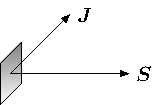
\includegraphics{figCapacitorCurrentFromCurrentDensityDotArea}
\caption{سطح سے گزرتی برقی رو۔}
\label{شکل_کپیسٹر_سطح_سے_گزرتی_برقی_رو}
\end{figure}

حل:چونکہ  یہاں \عددیء{\kvec{J}} مستقل مقدار ہے لہٰذا اسے مساوات \حوالہ{مساوات_کپیسٹر_برقی_رو_کثافت_کا_سطحی_تکمل_ہے} میں تکمل کے باہر لایا جا سکتا ہے اور یوں اس تکمل سے
\begin{align*}
I=\kvec{J} \cdot \kvec{S}= \SI{2}{\ampere}
\end{align*} 
حاصل ہوتا ہے۔برقی رو چونکہ مثبت ہے لہٰذا یہ سطح کی سمت میں ہی سطح سے گزر رہی ہے۔

اگر سطح کی دوسری طرف کو سطح کی سمت لی جائے تب \عددیء{\kvec{S}=-2\ax} لکھا جائے گا اور یوں
\begin{align*}
I=\kvec{J} \cdot \kvec{S}= \SI{-2}{\ampere}
\end{align*} 
حاصل ہو گا۔برقی رو کی مقدار اب بھی دو ایمپیئر ہی ہے البتہ اس کی علامت منفی ہے جس کا مطلب یہ ہے کہ برقی رو سطح کے سمت کی الٹی سمت میں ہے۔یوں اب بھی برقی رو بائیں سے دائیں ہی  گزر رہی ہے۔

\انتہا{مثال}
%

اس مثال سے آپ دیکھ سکتے ہیں کہ \عددیء{\kvec{S}} کی سمت میں برقی رو کو مثبت برقی رو کہا جاتا ہے۔
\begin{figure}
\centering
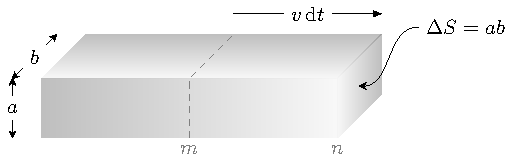
\includegraphics{figCapacitorPointFormOfOhmLaw}
\caption{حرکت کرتے چارج کی رفتار اور کثافت برقی رو۔}
\label{شکل_کپیسٹر_حرکت_کرتا_چارج_اور_کثافت_برقی_رو}
\end{figure}

شکل \حوالہ{شکل_کپیسٹر_حرکت_کرتا_چارج_اور_کثافت_برقی_رو} میں \عددیء{a} اور \عددیء{b} اطراف کی تار میں لمبائی کی سمت میں \عددیء{v} رفتار سے چارج حرکت کر رہا ہے۔شکل میں اس تار کا کچھ حصہ دکھایا گیا ہے۔یوں \عددیء{\dif t} دورانیہ میں چارج \عددیء{v \dif t} فاصلہ طے کرے گا۔اس طرح اس دورانیہ میں \عددیء{m} پر لگائی گئی نقطہ دار لکیر \عددیء{n} پہنچ جائے گی۔آپ دیکھ سکتے ہیں کہ اس دورانیہ میں \عددیء{m} اور \عددیء{n} کے درمیان موجود چارج سطح \عددیء{\Delta S} سے گزر جائے گا۔\عددیء{m} سے \عددیء{n} تک حجم \عددیء{a b v \dif t} کے برابر ہے۔اگر تار میں چارج کی حجمی کثافت \عددیء{\rho_h} ہو تب اس حجم میں  کُل چارج \عددیء{\rho_h a b v \dif t } ہو گا۔یوں برقی رو
\begin{align*}
I=\frac{\Delta Q}{\Delta t}=\frac{\rho_h a b v \dif t}{\dif t}=\rho_h \Delta S v
\end{align*}
لکھتے ہوئے  کثافت برقی رو
\begin{align*}
J=\frac{I}{\Delta S}=\rho_h v
\end{align*}
حاصل ہوتی ہے جس کی سمتی شکل
\begin{align}\label{مساوات_کپیسٹر_کثافت_رو_مساوی_کثافت_چارج_ضرب_رفتار}
\kvec{J}=\rho_h \kvec{v}
\end{align}
ہے۔اس مساوات میں \عددیء{\kvec{J}} \اصطلاح{کثافت اتصالی رو}\فرہنگ{کثافت رو!اتصالی}\فرہنگ{رو!کثافت اتصالی}\حاشیہب{convection current density}\فرہنگ{current!convection, density} کو ظاہر کرتی ہے۔

یہ مساوات کہتا ہے کہ حجمی چارج کثافت بڑھانے سے کثافت برقی رو اسی نسبت سے بڑھتی ہے۔اسی طرح چارج کی رفتار بڑھانے سے کثافت برقی رو اسی نسبت سے بڑھتی ہے۔یہ ایک عمومی نتیجہ ہے۔یوں سڑک پر زیادہ لوگ گزارنے کا ایک طریقہ انہیں تیز چلنے پر مجبور کرنے سے حاصل کیا جا سکتا ہے۔دوسرا طریقہ یہ ہے کہ انہیں قریب قریب کر دیا جائے۔ 


\حصہ{استمراری مساوات}
قانون بقائے چارج کہتا ہے کہ چارج کو نہ تو پیدا  اور نا ہی اسے ختم کیا جا سکتا ہے، اگرچہ برابر مقدار میں مثبت اور منفی چارج کو ملا کی انہیں ختم کیا جا سکتا ہے اور اسی طرح برابر مقدار میں انہیں پیدا بھی کیا جا سکتا ہے۔

یوں اگر ڈبے میں ایک جانب \عددیء{\SI{+5}{\coulomb}} اور دوسری جانب \عددیء{\SI{-3}{\coulomb}} چارج موجود ہو تو اس ڈبے میں کُل \عددیء{\SI{2}{\coulomb}} چارج ہے۔اگر ہم \عددیء{\SI{+3}{\coulomb}}  کو \عددیء{\SI{-3}{\coulomb}}  کے ساتھ ملا کر ختم کر دیں تب  بھی ڈبے میں کُل \عددیء{\SI{2}{\coulomb}} ہی چارج رہے گا۔

%=================
\ابتدا{مثال}
ایک ڈبہ جس کا حجم \عددیء{\SI{5}{\meter^3}} ہے میں حجمی کثافت چارج \عددیء{\SI{3}{\coulomb \per \meter^3}} ہے۔اس ڈبے سے چارج کی نکاسی ہو رہی ہے۔دو سیکنڈ میں حجمی کثافت چارج \عددیء{\SI{1}{\coulomb \per \meter^3}} رہ جاتی ہے۔ان دو سکینڈوں میں ڈبے سے خارج برقی رو کا تخمینہ لگائیں۔

حل:شروع میں ڈبے میں \عددیء{Q_1=3 \times 5=\SI{15}{\coulomb}} چارج ہے جبکہ دو سیکنڈ بعد اس میں \عددیء{Q_1=1 \times 5=\SI{5}{\coulomb}} رہ جاتا ہے۔یوں دو سیکنڈ میں ڈبے سے \عددیء{\SI{10}{\coulomb}} چارج خارج ہوتا ہے۔اس طرح  ڈبے سے خارج برقی رو \عددیء{\tfrac{10}{2}=\SI{5}{\ampere}} ہے۔اسی کو یوں لکھا جا سکتا ہے۔
\begin{align*}
I=-\frac{\Delta Q}{\Delta t}=-\frac{(5-15)}{2}=\SI{5}{\ampere}
\end{align*}
\انتہا{مثال}
%=======================

اس مثال میں آپ نے دیکھا کہ ڈبے میں \عددیء{\Delta Q} منفی ہونے کی صورت میں خارجی برقی رو کی قیمت مثبت ہوتی ہے۔آئیں اس حقیقت کو بہتر شکل دیں۔

حجم کو مکمل طور پر گھیرتی سطح کو بند سطح کہتے ہیں۔کسی بھی مقام پر ایسی سطح کی سمت سطح کے عمودی باہر کو ہوتی ہے۔مساوات \حوالہ{مساوات_کپیسٹر_برقی_رو_کثافت_کا_سطحی_تکمل_ہے} کے تحت برقی رو کو کثافت برقی رو کے سطحی تکمل سے بھی حاصل کیا جا سکتا ہے۔یوں
\begin{align}\label{مساوات_کپیسٹر_استمراری_مساوات_تکمل_شکل}
I=\oint_S \kvec{J} \cdot \dif \kvec{S}=-\frac{\dif Q}{\dif t}
\end{align}
لکھا جا سکتا ہے جہاں حجم کی سطح بند سطح ہونے کی بنا پر بند تکمل کی علامت استعمال کی گئی ہے اور \عددیء{Q} حجم میں کل چارج ہے۔

مساوات \حوالہ{مساوات_کپیسٹر_استمراری_مساوات_تکمل_شکل} \اصطلاح{استمراری مساوات}\فرہنگ{استمراری مساوات}\حاشیہب{continuity equation}\فرہنگ{continuity equation} کی تکمل شکل ہے۔آئیں اب اس کی نقطہ شکل حاصل کریں۔

مسئلہ پھیلاو کو صفحہ \حوالہصفحہ{مساوات_گاوس_مسئلہ_پھیلاو_تکمل_شکل} پر مساوات \حوالہ{مساوات_گاوس_مسئلہ_پھیلاو_تکمل_شکل} میں بیان کیا گیا ہے۔مسئلہ پھیلاو کسی بھی سمتی تفاعل کے لئے درست ہے لہٰذا اسے استعمال کرتے ہوئے مساوات \حوالہ{مساوات_کپیسٹر_استمراری_مساوات_تکمل_شکل} میں بند سطحی تکمل کو حجمی تکمل میں تبدیل کرتے ہیں۔
\begin{align*}
\oint_S \kvec{J} \cdot \dif \kvec{S}=\int_h (\nabla \cdot \kvec{J}) \dif h
\end{align*}
اگر حجم میں حجمی کثافت چارج \عددیء{\rho_h} ہو تب اس میں کل چارج
\begin{align*}
Q=\int_h \rho_h \dif h
\end{align*}
ہو گا۔ان دو نتائج کو استعمال کرتے ہوئے
\begin{align*}
\int_h (\nabla \cdot \kvec{J}) \dif h=-\frac{\dif}{\dif t} \int_h \rho_h \dif h
\end{align*}
لکھا جا سکتا ہے۔اس مساوات میں \عددیء{\tfrac{\dif}{\dif t}} دو متغیرات پر لاگو ہو گا۔یہ متغیرات تکمل کے اندر حجمی چارج کثافت \عددیء{\rho_h} اور حجم \عددیء{h} ہے۔

آپ جانتے ہیں کہ دو متغیرات کے تفرق کو جزوی تفرق کی شکل میں
\begin{align*}
\frac{\dif (uv)}{\dif t}=\frac{\partial u}{\partial t} v+ u  \frac{\partial v}{\partial t}
\end{align*}
لکھا جا سکتا ہے جہاں \عددیء{v} کو مستقل رکھتے ہوئے \عددیء{\tfrac{\partial u}{\partial t}} اور \عددیء{u} کو مستقل رکھتے ہوئے \عددیء{\tfrac{\partial v}{\partial t}} حاصل کیا جاتا ہے۔

اگر ہم یہ شرط لاگو کریں کہ حجم کی سطح تبدیل نہیں ہو گی تب حجم بھی تبدیل نہیں ہو گا اور یوں \عددیء{\tfrac{\dif}{\dif t}} کو جزوی تفرق میں تبدیل کرتے ہوئے تکمل کے اندر لکھتے ہوئے
\begin{align*}
\int_h (\nabla \cdot \kvec{J}) \dif h=\int_h -\frac{\partial \rho_h}{\partial t} \dif h
\end{align*}
حاصل ہوتا ہے۔یہ مساوات ہر ممکنہ حجم کے لئے درست ہے لہٰذا یہ نہایت چھوٹی حجم کے لئے بھی درست ہے۔نہایت چھوٹی حجم \عددیء{\dif h} کے لئے تکمل
\begin{align*}
 (\nabla \cdot \kvec{J}) \dif h= -\frac{\partial \rho_h}{\partial t} \dif h
\end{align*}
ہی ہے جس سے
\begin{align}\label{مساوات_کپیسٹر_استمراری_مساوات_نقطہ_شکل}
\nabla \cdot \kvec{J}=-\frac{\partial \rho_h}{\partial t}
\end{align}
حاصل ہوتا ہے۔مساوات \حوالہ{مساوات_کپیسٹر_استمراری_مساوات_نقطہ_شکل} استمراری مساوات کی نقطہ شکل ہے۔

پھیلاو کی تعریف کو ذہن میں رکھتے ہوئے آپ دیکھ سکتے ہیں کہ مساوات \حوالہ{مساوات_کپیسٹر_استمراری_مساوات_نقطہ_شکل} کہتا ہے کہ ہر نقطے پر چھوٹی سی حجم سے فی سیکنڈ چارج کا اخراج، یعنی برقی رو، فی اکائی حجم مساوی ہے چارج کے گھٹاو فی سیکنڈ فی اکائی حجم۔ 


\حصہ{موصل}
غیر چارج شدہ موصل میں منفی الیکٹران اور مثبت ساکن ایٹموں کی تعداد برابر ہوتی ہے البتہ اس میں برقی رو آزاد الیکٹران کے حرکت سے پیدا ہوتا ہے۔موصل میں الیکٹران آزادی سے بے ترتیب حرکت کرتا رہتا ہے۔یہ حرکت کرتا ہوا لمحہ بہ لمحہ ساکن ایٹم سے ٹکراتا ہے اور ہر ٹکر سے اس کے حرکت کی سمت تبدیل ہو جاتی ہے۔یوں ایسے الیکٹران کی اوسط رفتار صفر کے برابر ہوتی ہے۔آئیں دیکھیں کہ برقی میدان کے موجودگی میں کیا ہوتا ہے۔

برقی میدان \عددیء{\kvec{E}} میں الیکٹران پر قوت
\begin{align}
\kvec{F}=-e\kvec{E}
\end{align}
عمل کرے گی جہاں الیکٹران کا چارج \عددیء{-e} ہے۔ الیکٹران کی رفتار اس قوت کی وجہ سے  اسراع کے ساتھ قوت کی سمت میں بڑھنے شروع ہو جائے گی۔یوں بلا ترتیب رفتار  کے ساتھ ساتھ قوت کے سمت میں الیکٹران رفتار پکڑے گا۔موصل میں پائے جانے والا الیکٹران جلد کسی ایٹم سے ٹکرا جاتا ہے اور یوں اس کی سمت تبدیل ہو جاتی ہے۔جس لمحہ  الیکٹران کسی ایٹم سے ٹکراتا ہے اگر لاگو میدان کو صفر کر دیا جائے تو الیکٹران دوبارہ بلا ترتیب حرکت کرتا رہے گا اور اس کی اوسط رفتار دوبارہ صفر ہی ہو گی،  البتہ اس کی رفتار اب پہلے سے زیادہ ہو گی۔اگر الیکٹران ایٹم سے نہ ٹکراتا تب برقی میدان صفر کرنے کے بعد یہ برقرار قوت کی سمت میں حاصل کردہ رفتار سے حرکت کرتا رہتا۔یوں آپ دیکھ سکتے ہیں کہ ہر ٹکر سے الیکٹران کی اوسط رفتار صفر ہو جاتی ہے۔
اس طرح ہم دیکھتے ہیں کہ  \عددیء{\kvec{E}} کے موجودگی میں موصل میں الیکٹران کی رفتار مسلسل نہیں بڑھتی بلکہ یہ قوت کی سمت میں اوسط رفتار \عددیء{\kvec{v}_d} حاصل کرتا ہے اور جیسے ہی میدان صفر کر دیا جائے الیکٹران کی اوسط رفتار بھی صفر ہو جاتی ہے۔\عددیء{\kvec{v}_d} کو \اصطلاح{رفتار بہاو}\فرہنگ{رفتار بہاو}\حاشیہب{drift velocity}\فرہنگ{drift velocity} کہتے ہیں۔رفتار بہاو کا دارومدار \عددیء{\kvec{E}} کی قیمت پر ہے لہٰذا ہم
\begin{align}\label{مساوات_کپیسٹر_رفتار_بہاو}
\kvec{v}_d=-\mu_e \kvec{E}
\end{align}
لکھ سکتے ہیں جہاں مساوات کے مستقل \عددیء{\mu_e} کو الیکٹران کی \اصطلاح{حرکت پذیری}\فرہنگ{حرکت پذیری!الیکٹران}\حاشیہب{mobility}\فرہنگ{mobility!electron} کہتے ہیں۔حرکت پذیری کی مقدار مثبت ہے ۔چونکہ \عددیء{\kvec{v}_d} کو میٹر فی سیکنڈ اور \عددیء{\kvec{E}} کو وولٹ فی میٹر میں ناپا جاتا ہے لہٰذا حرکت پذیری کو \عددیء{\si{\meter \squared \per \volt \per \second}} میں ناپا جائے گا۔

مساوات \حوالہ{مساوات_کپیسٹر_رفتار_بہاو} کو صفحہ \حوالہصفحہ{مساوات_کپیسٹر_کثافت_رو_مساوی_کثافت_چارج_ضرب_رفتار} پر دئے مساوات \حوالہ{مساوات_کپیسٹر_کثافت_رو_مساوی_کثافت_چارج_ضرب_رفتار} میں پر کرتے ہوئے
\begin{align}
\kvec{J}=-\rho_e \mu_e \kvec{E}
\end{align}
حاصل ہوتا ہے جہاں موصل میں آزاد الیکٹران کی حجمی چارج کثافت کو \عددیء{\rho_e} لکھا گیا ہے۔\عددیء{\rho_e} منفی مقدار ہے۔یاد رہے کہ غیر چارج شدہ موصل میں حجمی کثافت چارج صفر کے برابر ہے چونکہ اس میں منفی الیکٹران  اور مثبت ایٹم کے چارج برابر ہوتے ہیں۔اس مساوات کو عموماً
\begin{align}\label{مساوات_کپیسٹر-اوہم_قانون_نقطہ_شکل}
\kvec{J}=\sigma \kvec{E}
\end{align}
لکھا جاتا ہے جو اوہم کے قانون\فرہنگ{قانون!اوہم}\فرہنگ{اوہم قانون!نقطہ شکل}\فرہنگ{Ohm's law!point form} کی نقطہ شکل ہے اور جہاں
\begin{align}\label{مساوات_کپیسٹر_موصلیت_تعریف}
\sigma=-\rho_e \mu_e
\end{align}
لکھا گیا ہے۔مساوات \حوالہ{مساوات_کپیسٹر-اوہم_قانون_نقطہ_شکل} میں \عددیء{\kvec{J}} کو \اصطلاح{کثافت ایصالی برقی رو} یا \عددیء{کثافت ایصالی رو}\فرہنگ{رو!کثافت ایصالی}\حاشیہب{conduction current density}\فرہنگ{current!density, conduction} ہے جبکہ \عددیء{\sigma} کو \اصطلاح{موصلیت کا مستقل}\فرہنگ{موصلیت!مستقل}\حاشیہب{conductivity}\فرہنگ{conductivity} کہتے ہیں اور اس کی اکائی\حاشیہد{یہ اکائی جرمنی کے جناب ارنسٹ ورنر وان سیمنز (1816-1892) کے نام ہے جنہوں نے موجودہ سیمنز ادارے کی بنیاد رکھی۔} سیمنز فی میٹر \عددیء{\si{\siemens \per \meter}} ہے۔سیمنز کو بڑے \عددیء{\si{\siemens}} سے  جبکہ سیکنڈ کو چھوٹے \عددیء{\second} سے ظاہر کیا جاتا ہے۔امید کی جاتی ہے کہ آپ ان میں غلطی نہیں کریں گے۔ اس کتاب کے آخر میں صفحہ  \حوالہصفحہ{جدول_جدول_موصلیت_کے_مستقل} پر جدول \حوالہ{جدول_جدول_موصلیت_کے_مستقل} میں کئی موصل اور غیر موصل اشیاء کی موصلیت پیش کی گئی ہیں۔
%================
\ابتدا{مثال}
تانبے\فرہنگ{تانبا}\حاشیہب{copper}\فرہنگ{copper} کی موصلیت کے مستقل  کی قیمت \عددیء{\SI{5.8e7}{\siemens \per \meter}} ہے جبکہ اس کی کمیتی کثافت \عددیء{\SI{8940}{\kilogram \per \meter^3}} اور ایٹمی کمیت \عددیء{\SI{63.5}{\gram}} ہیں۔اگر ہر ایٹم ایک عدد الیکٹران آزاد کرتا ہو تب تانبے میں الیکٹران کی حرکت پذیری حاصل کریں۔برقی میدان \عددیء{E=\SI{0.1}{\volt \per \meter}} کی صورت میں الیکٹران کا رفتار بہاو حاصل کریں۔

حل:ایٹمی کمیت \عددیء{\num{6.023e23}} یعنی ایک مول\حاشیہب{mole} ایٹم کی کمیت کو کہتے ہیں۔چونکہ ایک مربع میٹر میں \عددیء{\SI{8940}{\kilogram}} ہیں لہٰذا ایک مربع میٹر میں
\begin{align*}
\frac{8940 \times 6.023 \times 10^{23}}{0.0635}=8.48 \times 10^{28}
\end{align*} 
ایٹم پائیں جائیں گے۔ہر ایٹم ایک الیکٹران آزاد کرتا ہے لہٰذا \عددیء{\SI{0.1}{\nano \meter}} اطراف کے مربع میں اوسطاً \عددیء{0.848} یعنی تقریباً ایک عدد آزاد الیکٹران پایا جائے گا۔ اس طرح  ایک مربع میٹر میں کل آزاد الیکٹران چارج یعنی حجمی آزاد چارج کثافت
\begin{align}\label{مساوات_کپیسٹر_موصل_آزاد_چارج_کثافت}
\rho_e=-1.6 \times 10^{-19} \times 8.48 \times 10^{28}=\SI{-1.36e10}{\coulomb \per \meter^3}
\end{align}
ہو گی۔ایک مربع میٹر میں یوں انتہائی زیادہ آزاد چارج پایا جاتا ہے۔ اس طرح مساوات \حوالہ{مساوات_کپیسٹر_موصلیت_تعریف} کی مدد سے
\begin{align*}
\mu_e=-\frac{\sigma}{\rho_e}=\frac{5.8 \times 10^7}{-1.36 \times 10^{10}}=\SI{0.00427}{\meter \squared \per \volt \per \second}
\end{align*}
حاصل ہوتا ہے جہاں \عددیء{\SI{0.00427}{\meter \squared \siemens \per \coulomb}} کو \عددیء{\SI{0.00427}{\meter \squared \per \volt \per \second}} لکھا گیا ہے۔آپ تسلی کر سکتے ہیں کہ یہ برابر مقدار ہیں۔اب مساوات  \حوالہ{مساوات_کپیسٹر_رفتار_بہاو} استعمال کرتے ہوئے الیکٹران کی رفتار بہاو 
\begin{align*}
v_d = -0.00427 \times 0.1=\SI{-0.000427}{\meter \per \second}
\end{align*}
حاصل ہوتی ہے۔منفی رفتار کا مطلب ہے کہ الیکٹران \عددیء{\kvec{E}} کے الٹ سمت حرکت کر رہا ہے۔اس رفتار\حاشیہد{کھودا پہاڑ، نکلا چوہا۔آزاد الیکٹران تو کچھوے سے بھی آہستہ چلتا ہے۔} سے الیکٹران ایک کلو میٹر کا فاصلہ ستائیس دن و رات چل کر طے کرے گا۔یہاں یہ بتلاتا چلوں کہ عام درجہ حرارت مثلاً \عددیء{\SI{300}{\kelvin}} پر تانبے میں حرارتی توانائی سے حرکت کرتے الیکٹران کی رفتار تقریباً \عددیء{\SI{1000}{\kilo \meter \per \second}} ہوتی ہے۔

یوں موصل میں آزاد الیکٹرانوں کو نئی جگہ منتقل ہوتے  شہد کے مکھیوں کا جھنڈ  سمجھا جا سکتا ہے۔ایسے جھنڈ میں کوئی ایک مکھی نہایت تیز رفتار سے آگے پیچھے اڑتی ہے جبکہ پورا جھنڈ  نسبتاً آہستہ رفتار سے ایک سمت میں حرکت کرتا ہے۔موصل میں بھی کوئی ایک الیکٹران نہایت تیز رفتار سے ایٹموں سے ٹکراتا ہوا حرارتی توانائی کی وجہ سے  نہایت تیزی سے  اِدھر اُدھر حرکت کرتا ہے جبکہ بیرونی لاگو میدان کی وجہ سے ایسے تمام الیکٹران نہایت آہستہ رفتار سے میدان کی سمت میں حرکت کرتے ہیں۔

اگر موصل میں آزاد الیکٹران اتنے کم رفتار سے بیرونی لاگو میدان کی سمت میں صفر کرتے ہیں تب بجلی چالو کرتے ہی بلب  کس طرح روشن ہوتا ہے۔اس کو سمجھنے کی خاطر برقی تار کو پانی بھرے ایک لمبے  پائپ مانند سمجھیں۔ایسے پائپ میں جیسے ہی ایک جانب سے مزید پانی داخل کیا جائے، اسی وقت پائپ کے دوسرے سرے سے برابر پانی خارج ہو گا۔امید ہی سمجھ آ گئی ہو گی۔  
\انتہا{مثال}
%=============

مندرجہ بالا مثال میں بتلایا گیا کہ تانبے کا ہر ایٹم ایک عدد الیکٹران آزاد کرتا ہے۔اس حقیقت کو یوں سمجھا جا سکتا ہے کہ تانبے کا ایٹمی عدد \عددیء{29}ہے۔ایٹم کے کسی بھی مدار میں  \عددیء{2 n^2}  الیکٹران ہو سکتے ہیں جہاں پہلے مدار کے لئے \عددیء{n=1}، دوسرے مدار کے لئے \عددیء{n=2} وغیرہ لیا جاتا ہے۔یوں اس کے پہلے مدار میں \عددیء{2}، دوسرے مدار میں \عددیء{8}، تیسرے مدار میں \عددیء{18} اور آخری مدار\حاشیہد{چوتھے مدار میں \عددیء{32} الیکٹران ممکن ہیں لیکن تانبے کے ایٹم میں اس مدار کے لئے صرف ایک عدد الیکٹران بچتا ہے۔} میں \عددیء{1} الیکٹران ہو گا۔ایٹم آخری مدار میں واحد الیکٹران کو آزاد کرتا ہے۔آئیں اب بڑی شکل میں اوہم کا قانون حاصل کریں۔ 
\begin{figure}
\centering
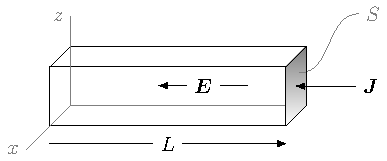
\includegraphics{figCapacitorOhmLawFromPointForm}
\caption{اوہم کے قانون کی بڑی شکل۔}
\label{شکل_کپیسٹر_اوہم_قانون_بڑی_شکل}
\end{figure}

شکل \حوالہ{شکل_کپیسٹر_اوہم_قانون_بڑی_شکل} میں  موصل سلاخ دکھایا گیا ہے جس کی لمبائی \عددیء{L} اور  رقبہ عمودی تراش \عددیء{S} ہیں۔سلاخ کو \عددیء{\ay} سمت میں لیٹا تصور کریں۔سلاخ میں لمبائی کی سمت میں مستقل اور یکساں برقی میدان \عددیء{\kvec{E}=-E\ay}  اور کثافت برقی رو \عددیء{\kvec{J}=-J\ay} پائے جاتے ہیں۔یوں اگر سلاخ کا بایاں سرا برقی زمین تصور کیا جائے تب اس کے دائیں سرے پر برقی دباو کو صفحہ \حوالہصفحہ{مساوات_توانائی_برقی_دباو_تعریف} پر دئے مساوات \حوالہ{مساوات_توانائی_برقی_دباو_تعریف} سے یوں
\begin{align*}
V= -\int_0^L \kvec{E} \cdot \dif \kvec{L}=\int_0^L E \ay \cdot \dif  y \ay=\int_0^L E \dif y=E\int_0^L \dif y=EL
\end{align*}
حاصل کرتے ہیں۔رقبہ عمودی تراش کو شکل میں گہرے رنگ سے اجاگر کیا گیا ہے۔سمتی رقبہ عمودی تراش بند سطح نہیں ہے لہٰذا اس کے دو ممکنہ رخ ہیں۔سلاخ کے دائیں سرے سے داخل برقی رو حاصل کرنے کی غرض سے رقبہ عمودی تراش کو \عددیء{\kvec{S}=-S\ay} لکھتے ہیں۔یوں دائیں سرے سے داخل برقی رو کی مقدار مثبت ہو گی۔برقی رو
\begin{align*}
I=\int_S \kvec{J} \cdot \dif \kvec{S}=JS
\end{align*}
حاصل ہوتی ہے۔ان معلومات کو شکل \حوالہ{مساوات_کپیسٹر-اوہم_قانون_نقطہ_شکل} میں پُر کرتے ہوئے
\begin{align*}
\frac{I}{S}=\sigma \frac{V}{L}
\end{align*}
  یا
\begin{align*}
V=I \frac{L}{\sigma S}
\end{align*}
حاصل ہوتا ہے جہاں
\begin{align}\label{مساوات_کپیسٹر_سلاخ_کی_مزاحمت}
R= \frac{L}{\sigma S}
\end{align}
کو مزاحمت لکھتے ہوئے
\begin{align}\label{مساوات_کپیسٹر_اوہم_قانون_بڑی_شکل}
V=IR
\end{align}
حاصل ہوتا ہے جو اوہم کے قانون\فرہنگ{اوہم!قانون}\فرہنگ{Ohm's law} کی جانی پہچانی شکل ہے۔

مساوات \حوالہ{مساوات_کپیسٹر_سلاخ_کی_مزاحمت} یکساں رقبہ عمودی تراش رکھنے والے موصل سلاخ کی \اصطلاح{مزاحمت}\فرہنگ{مزاحمت}\حاشیہب{resistance}\فرہنگ{resistance} دیتا ہے جہاں مزاحمت کی اکائی \اصطلاح{اوہم}\فرہنگ{اوہم}\حاشیہب{ohm}\فرہنگ{ohm} ہے جسے \عددیء{\si{\ohm}} سے ظاہر کیا جاتا ہے۔یکساں رقبہ عمودی تراش کے سلاخ میں برقی میدان یکساں ہوتا ہے۔اگر سلاخ کا رقبہ عمودی تراش یکساں نہ ہو تب اس میں برقی میدان بھی یکساں نہ ہو گا اور ایسی صورت میں مساوات \حوالہ{مساوات_کپیسٹر_سلاخ_کی_مزاحمت} استعمال نہیں کیا جا سکتا البتہ ایسی صورت میں بھی مزاحمت کو مساوات \حوالہ{مساوات_کپیسٹر_اوہم_قانون_بڑی_شکل} کی مدد سے برقی دباو فی اکائی برقی رو سے بیان کیا جاتا ہے۔یوں مساوات \حوالہ{مساوات_توانائی_برقی_دباو_تعریف} اور مساوات \حوالہ{مساوات_کپیسٹر_برقی_رو_کثافت_کا_سطحی_تکمل_ہے} استعمال کرتے ہوئے سلاخ کے  \عددیء{b} سے \عددیء{a} سرے تک مزاحمت
\begin{align}\label{مساوات_کپیسٹر_مزاحمت_کی_عمومی_مساوات}
R=\frac{V}{I}=\frac{-\int \limits_b^a \kvec{E} \cdot \dif \kvec{L}}{\int \limits_S \kvec{J} \cdot \dif \kvec{S}}=\frac{-\int \limits_b^a \kvec{E} \cdot \dif \kvec{L}}{\int \limits_S \sigma \kvec{E} \cdot \dif \kvec{S}}
\end{align} 
سے حاصل ہو گی جہاں برقی رو سلاخ کے مثبت برقی دباو والے سرے سے سلاخ میں داخل ہوتے برقی رو کو کہتے ہیں۔یوں مندرجہ بالا مساوات میں سطحی تکمل سلاخ کے مثبت سرے پر حاصل کیا جائے گا جہاں سطح عمودی تراش کی سمت سلاخ کی جانب لی جائے گی۔
%=============
\ابتدا{مثال}
تانبے کی ایک کلو میٹر لمبی اور تین ملی میٹر رداس کے تار کی مزاحمت حاصل کریں۔

حل:یہاں \عددیء{L=\SI{1000}{\meter}} جبکہ \عددیء{S=\pi r^2=\SI{2.83e-7}{\meter \squared}} اور \عددیء{\sigma=5.8\times 10^7} ہے لہٰذا
\begin{align*}
R=\frac{1000}{5.8\times 10^7 \times 2.83 \times 10^{-7}}=\SI{0.61}{\ohm}
\end{align*}
حاصل ہوتا ہے۔
\انتہا{مثال}

%=============
\ابتدا{مشق}
المونیم میں کثافت برقی رو مندرجہ ذیل صورتوں میں حاصل کریں۔( الف) برقی میدان کی شدت \عددیء{\SI{50}{\milli \volt \per \meter}} ہے۔ (ب) آزاد الیکٹران کی رفتار بہاو \عددیء{\SI{0.12}{\milli \meter \per \second}} ہے۔ (پ) ایک ملی میٹر موٹی تار جس میں \عددیء{\SI{2}{\ampere}} برقی رو گزر رہی ہے۔

جوابات:\عددیء{\SI{1.91}{\mega \ampere \per \meter \squared}}،  \عددیء{\SI{3.82}{\mega \ampere \per \meter \squared}} اور \عددیء{\SI{2.55}{\mega \ampere \per \meter \squared}}
\انتہا{مشق}
%===============================

ہم دیکھ چکے ہیں کہ موصل کے اندر داخل کیا گیا چارج  جلد موصل کے سطح پر پہنچ کر سطحی چارج کثافت پیدا کرتا ہے۔یہ جانتے ہوئے کہ حقیقت میں موصل کے اندر چارج کا پیدا ہونا یا وہاں چارج داخل کرنا معمول کی بات ہرگز نہیں، ہم ایسے داخل کئے گئے چارج کی حرکت پر غور کرتے ہیں۔

اوہم کے قانون
\begin{align*}
\kvec{J}=\sigma \kvec{E}
\end{align*}
اور استمراری مساوات
\begin{align*}
\nabla \cdot \kvec{J}=-\frac{\partial \rho_h}{\partial t}
\end{align*} 
دونوں میں صرف آزاد چارج کی بات کی جاتی ہے۔ان مساوات سے
\begin{align*}
\nabla \cdot \sigma \kvec{E}=-\frac{\partial \rho_h}{\partial t}
\end{align*} 
یا
\begin{align*}
\nabla \cdot \frac{\sigma}{\epsilon} \kvec{D}=-\frac{\partial \rho_h}{\partial t}
\end{align*} 
لکھا جا سکتا ہے۔اگر موصل میں \عددیء{\sigma} اور \عددیء{\epsilon} کی قیمتیں اٹل ہوں تب اس مساوات کو
\begin{align*}
\nabla \cdot  \kvec{D}=-\frac{\epsilon}{\sigma}\frac{\partial \rho_h}{\partial t}
\end{align*} 
لکھا جا سکتا ہے۔صفحہ \حوالہصفحہ{مساوات_گاوس_میکسویل_پہلی_مساوات_نقطہ_شکل} پر مساوات \حوالہ{مساوات_گاوس_میکسویل_پہلی_مساوات_نقطہ_شکل} جو میکس ویل کی پہلی مساوات ہے کی مدد سے یوں
\begin{align*}
\rho_h=-\frac{\epsilon}{\sigma}\frac{\partial \rho_h}{\partial t}
\end{align*} 
حاصل ہوتا ہے۔مساوات \حوالہ{مساوات_کپیسٹر_موصلیت_تعریف} کہتا ہے کہ موصلیت کی قیمت آزاد الیکٹران کی حجمی چارج کثافت \عددیء{\rho_e} اور الیکٹران کی حرکت پذیری پر منحصر ہے۔مساوات \حوالہ{مساوات_کپیسٹر_موصل_آزاد_چارج_کثافت} تانبے میں \عددیء{\rho_e=\SI{-1.36e10}{\coulomb \per \meter^3}} دیتا ہے جو انتہائی بڑی مقدار ہے۔اتنے چارج میں بیرونی داخل چارج نمک برابر بھی حیثیت نہیں رکھتا لہٰذا \عددیء{\sigma} کی قیمت کو اٹل تصور کیا جا سکتا ہے۔ یوں مندرجہ بالا مساوات کو نئی شکل
\begin{align*}
\frac{\partial \rho_h}{\rho_h}=-\frac{\sigma}{\epsilon} \partial t
\end{align*} 
میں لکھتے ہوئے، اس کا تکمل
\begin{align*}
\rho_h=\rho_0 e^{-\frac{\sigma}{\epsilon}t}
\end{align*}
 حاصل کرتے ہیں جہاں وقت \عددیء{t=0} پر داخل کئے گئے چارج کا حجمی چارج کثافت \عددیء{\rho_0} ہے۔اس مساوات کے تحت حجمی چارج کثافت \عددیء{\tfrac{\sigma}{\epsilon}} \اصطلاح{وقتی مستقل}\فرہنگ{وقتی مستقل}\حاشیہب{time constant}\فرہنگ{time constant} رکھتا ہے۔تقطیر شدہ پانی کا وقتی مستقل جدول \حوالہ{جدول_جدول_موصلیت_کے_مستقل} اور جدول \حوالہ{جدول_جدول_جزوی_برقی_مستقل_زاویہ_زیاع} کی مدد سے
\begin{align*}
\frac{\epsilon}{\sigma}=\frac{80}{36 \pi \times 10^9 \times 10^{-4}}=\SI{7.07}{\micro \second}
\end{align*}
حاصل ہوتا ہے۔اگرچہ تقطیر شدہ پانی انتہائی کم موصل ہے لیکن اس میں بھی  کثافت چارج صرف سات مائیکرو سیکنڈ میں ابتدائی قیمت کے صرف \عددیء{37}  فی صد رہ جاتا ہے۔یوں کسی بھی موصل کے اندر انتہائی کم دورانیے کے لئے اضافی چارج پایا جا سکتا ہے۔اس لمحاتی چارج کثافت کے علاوہ اندرون موصل  کو چارج سے پاک تصور کیا جا سکتا ہے۔

ذو برق میں مختلف وجوہات کی بنا پر لگاتار آزاد چارج پیدا ہوتے رہتے ہیں جس کی بنا پر ذو برق صفر سے زیادہ موصلیت رکھتے ہوئے برقی رو گزارتا ہے۔ذو برق کے اندر چارج بھی آخر کار سطح پر پہنچ جاتا ہے۔




\حصہ{موصل کے خصوصیات اور سرحدی شرائط}
غیر چارج شدہ موصل میں کُل آزاد الیکٹران اور مثبت ایٹم برابر تعداد میں پائے جاتے ہیں۔یوں اس میں برقی میدان صفر کے برابر ہوتا ہے۔فرض کریں کہ غیر چارج شدہ موصل کے اندر کسی طرح چند الیکٹران نمودار ہو جاتے ہیں۔یہ الیکٹران برقی میدان \عددیء{\kvec{E}} پیدا کریں گے جس کی وجہ سے  موصل میں آزاد الیکٹران  موصل کے سطح کی جانب چل پڑیں گے۔سطح کے باہر غیر موصل خلاء پائی جاتی ہے جس میں الیکٹران حرکت نہیں کر سکتے لہٰذا الیکٹران موصل کے سطح پر پہنچ کر رک جائیں گے۔موصل میں نمودار ہونے والے الیکٹران کے برابر تعداد میں الیکٹران موصل کے سطح پر منتقل ہوں گے جس کے بعد موصل میں دوبارہ منفی الیکٹران اور مثبت ایٹموں کی تعداد برابر ہو جائے گی اور یہ غیر چارج شدہ صورت اختیار کر لے گا۔

آپ نے دیکھا کہ اضافی  چارج موصل میں زیادہ دیر نہیں رہ سکتا اور یہ جلد  سطح پر منتقل ہو جاتا ہے۔یوں اضافی چارج  موصل  کے سطح پر بیرونی جانب چمٹا رہتا ہے۔یہ موصل کی پہلی اہم خاصیت ہے۔

موصل کی دوسری خاصیت \اصطلاح{برقی سکون}\فرہنگ{برقی سکون}\حاشیہب{electrostatic}\فرہنگ{electrostatic} کی حالت کے لئے بیان کرتے ہیں۔برقی سکون سے مراد ایسی صورت ہے جب چارج حرکت نہ کر رہا ہو یعنی جب برقی رو صفر کے برابر ہو۔برقی سکون کی حالت میں موصل کے اندر ساکن برقی میدان صفر رہتا ہے۔اگر ایسا نہ ہوتا تو میدان کی وجہ سے اس میں آزاد الیکٹران حرکت کر کے برقی رو کو جنم دیتے جو غیر ساکن حالت ہے۔

یوں برقی سکون کی حالت میں موصل کے اندر اضافی چارج اور برقی میدان دونوں صفر کے برابر ہوتے ہیں البتہ اس کے سطح پر بیرونی جانب چارج پایا جا سکتا ہے۔آئیں دیکھیں کہ سطح پر پائے جانے والا چارج موصل کے باہر کس قسم کا برقی میدان پیدا کرتا ہے۔

موصل کے سطح پر چارج، موصل کے باہر برقی میدان پیدا کرتا ہے۔سطح پر کسی بھی نقطے پر ایسے میدان کو دو اجزاء کے مجموعے کی شکل میں لکھا جا سکتا ہے۔پہلا جزو سطح کے مماسی  اور دوسرا جزو سطح کے عمودی رکھتے ہوئے ہم دیکھتے ہیں کہ مماسی جزو صفر ہو گا۔اگر ایسا نہ ہو تو اس میدان کی وجہ سے سطح پر پائے جانے والے آزاد الیکٹران حرکت میں آئیں گے جو غیر ساکن حالت ہو گی۔یوں ہم
\begin{align}
E_{\textup{مماسی}}=0
\end{align}
لکھ سکتے ہیں۔سطح پر عمودی برقی میدان گاوس کے قانون کی مدد سے حاصل کیا جا سکتا ہے جو کہتا ہے کہ کسی بھی بند سطح سے کُل برقی بہاو کا اخراج، سطح میں گھیرے چارج کے برابر ہوتا ہے۔چونکہ سطح پر مماسی برقی میدان صفر ہے اور موصل کے اندر بھی برقی میدان صفر ہے لہٰذا سطح پر چارج سے برقی بہاو کا اخراج صرف عمودی سمت میں ہو سکتا ہے۔یوں \عددیء{\Delta S} سطح سے عمودی اخراج \عددیء{D \Delta S} اسی سطح پر چار \عددیء{\rho_S \Delta S} کے برابر ہو گا جس سے
\begin{align}\label{مساوات_کپیسٹر_عمودی_میدان_برابر_کثافت_چارج}
D_{\textup{عمودی}}=\rho_S
\end{align} 
حاصل ہوتا ہے۔آئیں اسی بحث کو بہتر جامہ پہنائیں۔ایسا کرتے ہوئے ہم ایک عمومی ترکیب سیکھ لیں گے جو مختلف اقسام کے اشیاء کے سرحد پر میدان کے حصول کے لئے استعمال کیا جاتا ہے۔  

\begin{figure}
\centering
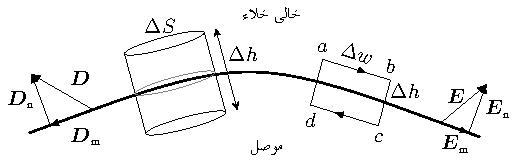
\includegraphics{figCapacitorElectricFieldConductorAirBoundaryCondition}
\caption{موصل اور خلاء کے سرحد پر برقی شرائط۔}
\label{شکل_کپیسٹر_موصل_خلاء_برقی_شرائط}
\end{figure}

شکل \حوالہ{شکل_کپیسٹر_موصل_خلاء_برقی_شرائط} میں موصل اور خالی خلاء کے درمیان سرحد موٹی لکیر سے دکھایا گیا ہے۔اس سرحد پر خلاء میں \عددیء{\kvec{E}} اور \عددیء{\kvec{D}} دکھائے گئے ہیں۔خلاء میں \عددیء{\kvec{E}} کو \عددیء{\kvec{E}_m} اور \عددیء{\kvec{E}_n} کے مجموعے کے طور پر بھی دکھایا گیا ہے جو بالترتیب سرحد کے مماسی اور عمودی اجزاء ہیں۔اسی طرح \عددیء{\kvec{D}} کو بھی مماسی اور عمودی اجزاء کے مجموعہ کے طور پر دکھایا گیا ہے۔ہم صرف اس حقیقت کو لے کر آگے بڑھتے ہیں کہ موصل کے اندر \عددیء{\kvec{E}} اور \عددیء{\kvec{D}} دونوں صفر کے برابر ہیں۔آئیں اس حقیقت کی بنا پر خلاء میں   \عددیء{\kvec{E}} کی قیمت حاصل کریں۔ہم \عددیء{\kvec{E}} کے مجموعے  \عددیء{\kvec{E}_m} اور \عددیء{\kvec{E}_n} حاصل کریں گے۔پہلے \عددیء{\kvec{E}_m} حاصل کرتے ہیں۔ 

 سرحد پر \عددیء{abcd}  مستطیل بنایا گیا ہے جہاں \عددیء{ab} اور \عددیء{cd} سرحد کے مماسی جبکہ \عددیء{bc} اور \عددیء{da} سرحد کے عمودی ہیں۔\عددیء{ab} خالی خلاء میں سرحد سے \عددیء{\Delta h /2} فاصلے پر جبکہ \عددیء{cd} موصل میں سرحد سے  \عددیء{\Delta h /2} فاصلے پر  ہیں۔\عددیء{ab} اور \عددیء{cd} کی لمبائیاں \عددیء{\Delta w} ہیں جبکہ \عددیء{bc} اور \عددیء{da} کی لمبائیاں \عددیء{\Delta h} ہے۔صفحہ \حوالہصفحہ{مساوات_توانائی_بند_راستا} پر دئے مساوات \حوالہ{مساوات_توانائی_بند_راستا} 
\begin{align*}
\oint \kvec{E} \cdot \dif \kvec{L}=0
\end{align*}
کو \عددیء{abcd} پر  لاگو کرتے ہیں۔اس تکمل کو چار ٹکڑوں کا مجموعہ لکھا جا سکتا ہے۔
   \begin{align*}
\oint \kvec{E} \cdot \dif \kvec{L}=\int_a^b \kvec{E} \cdot \dif \kvec{L}+\int_b^c \kvec{E} \cdot \dif \kvec{L}+\int_c^d \kvec{E} \cdot \dif \kvec{L}+\int_d^a \kvec{E} \cdot \dif \kvec{L}=0
\end{align*}
اب \عددیء{a} سے \عددیء{b} تک
\begin{align*}
\int_a^b\kvec{E} \cdot \dif \kvec{L}=E_m \Delta w
\end{align*}
حاصل ہوتا ہے۔خلاء میں نقطہ \عددیء{b}  پر عمودی میدان کو \عددیء{E_{n,b}} لکھتے ہوئے \عددیء{b} سے \عددیء{c} تک
\begin{align*}
\int_b^c\kvec{E} \cdot \dif \kvec{L}=-E_{n,b} \frac{\Delta h}{2}
\end{align*}
حاصل ہوتا ہے۔یاد رہے کہ \عددیء{bc} کی آدھی لمبائی موصل کے اندر ہے جہاں \عددیء{\kvec{E}=0} ہے۔\عددیء{c} سے \عددیء{d} تک تکمل صفر کے برابر ہے چونکہ یہ راستہ موصل کے اندر ہے جہاں \عددیء{\kvec{E}=0} ہے۔
\begin{align*}
\int_c^d\kvec{E} \cdot \dif \kvec{L}=0
\end{align*}
خلاء میں نقطہ \عددیء{a}  پر عمودی میدان کو \عددیء{E_{n,a}} لکھتے ہوئے \عددیء{d} سے \عددیء{a} تک
\begin{align*}
\int_d^a\kvec{E} \cdot \dif \kvec{L}=E_{n,a} \frac{\Delta h}{2}
\end{align*}
ان چار نتائج سے
\begin{align*}
\oint \kvec{E} \cdot \dif \kvec{L}=E_m \Delta w+\left(E_{n,a}-E_{n,b} \right) \frac{\Delta h}{2}=0
\end{align*}
لکھا جا سکتا ہے۔سرحد کے قریب میدان حاصل کرنے کی خاطر ہمیں سرحد کے قریب تر ہونا ہو گا یعنی \عددیء{\Delta h} کو تقریباً صفر کے برابر کرنا ہو گا۔ایسا کرنے
 سے \عددیء{(E_{n,a}-E_{n,b})\tfrac{\Delta h}{2}} کو نظرانداز  کیا جا سکتا ہے۔ہم \عددیء{\Delta w} کو اتنا چھوٹا لیتے ہیں کہ اس کی پوری لمبائی پر میدان کو یکساں تصور کرنا ممکن ہو۔ایسا کرتے ہوئے اس مساوات سے
\begin{align*}
\oint \kvec{E} \cdot \dif \kvec{L}=E_m \Delta w=0
\end{align*}
یعنی
\begin{align}\label{مساوات_کپیسٹر_سرحد_موصل_خلاء_مماسی_میدان_صفر}
E_m=0
\end{align}
حاصل ہوتا ہے۔آئیں اب \عددیء{E_n} حاصل کریں۔\عددیء{E_n} کی بجائے گاوس کے قانون
\begin{align*}
\oint_S \kvec{D} \cdot \dif \kvec{S}=Q
\end{align*}
 کی مدد سے \عددیء{D_n} کا حصول زیادہ آسان ثابت ہوتا ہے لہٰذا ہم اسی کو حاصل کرتے ہیں۔

شکل \حوالہ{شکل_کپیسٹر_موصل_خلاء_برقی_شرائط} میں موصل اور خالی خلاء کے سرحد پر \عددیء{\Delta h} لمبائی کا بیلن دکھایا گیا ہے۔اس بیلن کے ڈھکنوں کا رقبہ \عددیء{\Delta S} ہے۔اگر سرحد پر \عددیء{\rho_S} پایا جائے تب بیلن \عددیء{\rho_S \Delta S} چارج کو گھیرے گا۔گاوس کے قانون کے تحت بیلن سے اسی مقدار کے برابر برقی بہاو کا اخراج ہو گا۔برقی بہاو کا اخراج بیلن کے دونوں سروں اور اس کے نلکی نما سطح سے ممکن ہے۔یوں
\begin{align*}
\oint \limits_S \kvec{D} \cdot \dif \kvec{S}=\int \limits_{\textup{نچلا ڈھکن}} \kvec{D} \cdot \dif \kvec{S}+\int \limits_{\textup{بالائی ڈھکن}} \kvec{D} \cdot \dif \kvec{S}+\int \limits_{\textup{نلکی سطح}} \kvec{D} \cdot \dif \kvec{S}=\rho_S \Delta S
\end{align*}
لکھا جا سکتا ہے۔اب بیلن کی نچلی سطح موصل کے اندر ہے جہاں میدان صفر کے برابر ہے لہٰذا
\begin{align*}
\int \limits_{\textup{نچلا ڈھکن}} \kvec{D} \cdot \dif \kvec{S}=0
\end{align*}
ہو گا۔مساوات \حوالہ{مساوات_کپیسٹر_سرحد_موصل_خلاء_مماسی_میدان_صفر} کے تحت سرحد پر خلاء میں مماسی میدان صفر ہوتا ہے۔موصل میں بھی میدان صفر ہوتا ہے لہٰذا  
\begin{align*}
\int \limits_{\textup{نلکی سطح}} \kvec{D} \cdot \dif \kvec{S}=0
\end{align*}
ہو گا۔بیلن کے بالائی سرے پر
\begin{align*}
\int \limits_{\textup{بالائی ڈھکن}} \kvec{D} \cdot \dif \kvec{S}=D_n \Delta S
\end{align*}
ہو گا۔ان تین نتائج کو استعمال کرتے ہوئے
\begin{align*}
\oint_S \kvec{D} \cdot \dif \kvec{S}=D_n \Delta S=\rho_S \Delta S
\end{align*}
یعنی
\begin{align*}
D_n=\rho_S
\end{align*}
حاصل ہوتا ہے۔چونکہ \عددیء{D=\epsilon_0 E} ہوتا ہے لہٰذا یوں 
\begin{align}\label{مساوات_کپیسٹر_سرحد_موصل_خلاء_عمودی_میدان}
D_n=\epsilon_0 E_n=\rho_S
\end{align}
لکھا جا سکتا ہے۔

مساوات \حوالہ{مساوات_کپیسٹر_سرحد_موصل_خلاء_مماسی_میدان_صفر} اور مساوات \حوالہ{مساوات_کپیسٹر_سرحد_موصل_خلاء_عمودی_میدان} موصل اور خالی خلاء کے سرحد پر برقی میدان کے شرائط بیان کرتے ہیں۔موصل اور خلاء کے سرحد پر برقی میدان موصل سے عمودی خارج ہوتا ہے جبکہ اس کے سرحد کے مماسی میدان صفر کے برابر ہوتا ہے۔نتیجتاً موصل کی سطح \اصطلاح{ہم قوہ سطح} ہوتی ہے۔یوں موصل کی سطح پر دو نقطوں کے مابین کسی بھی راستے پر برقی میدان کا تکمل صفر کے برابر ہو گا یعنی \عددیء{\int_a^b \kvec{E} \cdot \dif \kvec{L}=0} ہو گا۔یاد رہے کہ برقی میدان کا تکمل برقی دباو دیتا ہے جو تکمل کے راستے پر منحصر نہیں ہوتا لہٰذا اس راستے کو موصل کی سطح پر ہی رکھا جا سکتا ہے جہاں \عددیء{\kvec{E}_{\textup{مماسی}}=0} ہونے کی وجہ سے تکمل صفر کے برابر ہو گا۔ 
%===============

\ابتدا{مشق}
نقطہ \عددیء{N(2,-3,5)} موصل کی سطح پر پایا جاتا ہے جہاں \عددیء{\kvec{E}=210\ax-350\ay+99\az \, \si{\volt \per \meter}} کے برابر ہے۔اس نقطے  پر \عددیء{E_m}، \عددیء{E_n} اور \عددیء{\rho_S} حاصل کریں۔

جوابات:0، \عددیء{\SI{420}{\volt \per \meter}} اور \عددیء{\SI{3.71}{\nano \coulomb \per \meter \squared}}
\انتہا{مشق}
%==================

\حصہ{عکس کی ترکیب}
جفت قطب کے خطوط صفحہ \حوالہصفحہ{شکل_توانائی_جفت_قطب_ہم_قوہ_اور_سمت_بہاو_خط} پر  شکل \حوالہ{شکل_توانائی_جفت_قطب_ہم_قوہ_اور_سمت_بہاو_خط} میں دکھائے گئے ہیں جہاں دونوں چارجوں سے برابر فاصلے پر لامحدود برقی زمینی سطح دکھائی گئی ہے۔برقی زمین پر انتہائی باریک موٹائی کی لامحدود موصل سطح رکھی جا سکتی ہے۔ایسی موصل سطح پر برقی دباو صفر وولٹ ہو گا اور اس پر میدان عمودی ہو گا۔موصل کے اندر برقی میدان صفر رہتا ہے اور اس سے برقی میدان گزر نہیں پاتا۔

اگر اس موصل سطح کے نیچے سے جفت قطب کا منفی چارج ہٹا دیا جائے تب بھی سطح کے بالائی جانب میدان عمودی ہی ہو گا۔یاد رہے برقی زمین صفر وولٹ پر ہوتی ہے۔موصل سطح سے اوپر میدان جوں کا توں رہے گا جبکہ اس سے نیچے میدان صفر ہو جائے گا۔اسی طرح سطح سے اوپر  جفت قطب کا مثبت چارج ہٹانے سے سطح کے نچلے میدان پر کوئی اثر نہیں پڑتا جبکہ سطح سے اوپر میدان صفر ہو جاتا ہے۔

آئیں ان حقائق کو دوسری نقطہ نظر سے دیکھیں۔فرض کریں کہ لامحدود موصل سطح یا برقی زمین سے \عددیء{\tfrac{d}{2}} فاصلے پر  اوپر مثبت نقطہ چارج \عددیء{+Q} پایا جاتا ہے۔چونکہ ایسی صورت میں سطح سے اوپر برقی میدان بالکل جفت قطب کے میدان کی طرح ہو گا لہٰذا ہم \عددیء{\tfrac{d}{2}} فاصلے پر برقی زمین سے نیچے عین مثبت چارج کے نیچے منفی چارج \عددیء{-Q} رکھتے ہوئے برقی زمین کو ہٹا سکتے ہیں۔اوپر جانب کے میدان پر ان اقدام کا کوئی اثر نہیں ہو گا۔یوں جفت قطب کے تمام مساوات بروئے کار لاتے ہوئے زمین کے اوپر جانب کا میدان حاصل کیا جا سکتا ہے۔یاد رہے کہ سطح کے نیچے برقی زمین کو صفر ہی تصور کیا جائے گا۔اگر برقی زمین کی سطح کو آئینہ تصور کیا جائے تب مثبت چارج کا عکس اس آئینہ میں اسی مقام پر نظر آئے گا جہاں ہم نے تصوراتی منفی چارج رکھا۔یوں اس منفی چارج کو حقیقی چارج کا \اصطلاح{عکس}\فرہنگ{عکس}\حاشیہب{image}\فرہنگ{image} کہتے ہیں۔

ایسی ہی ترکیب لامحدود زمینی سطح کے ایک جانب منفی چارج سے پیدا میدان حاصل کرنے کی خاطر بھی استعمال کیا جاتا ہے۔ایسی صورت میں زمین کی دوسری جانب عین منفی چارج کے سامنے،  اتنے ہی فاصلے پر برابر مقدار مگر مثبت چارج رکھتے ہوئے برقی زمین کو ہٹایا جا سکتا ہے۔

کسی بھی چارج کو نقطہ چارجوں کا مجموعہ تصور کیا جا سکتا ہے۔لہٰذا لامحدود برقی زمین یا لامحدود موصل سطح  کی ایک جانب کسی بھی شکل کے چارجوں  کا میدان، سطح کی دوسری جانب چارجوں کا عکس رکھتے اور زمین کو ہٹاتے ہوئے حاصل کیا جاتا ہے۔اس ترکیب کو \اصطلاح{عکس کی ترکیب}\فرہنگ{عکس کی ترکیب} کہتے ہیں۔یاد رہے کہ کسی بھی لامحدود موصل سطح جس کے ایک جانب چارج پایا جاتا ہو پر سطحی چارج پایا جائے گا۔عموماً مسئلے میں لامحدود سطح اور سطح کے باہر چارج معلوم ہوں گے۔ایسے مسئلے کو حل کرنے کی خاطر سطح پر سطحی چارجوں کا علم بھی ضروری ہوتا ہے۔سطحی چارج دریافت کرنا نسبتاً مشکل کام ہے جس سے چھٹکارا حاصل کرنا عقلمندی ہو گی۔عکس کی ترکیب میں سطحی چارج کا جاننا ضروری نہیں لہٰذا اس ترکیب سے مسئلہ کو حل کرنا عموماً زیادہ آسان ثابت ہوتا ہے۔
\begin{figure}
\centering
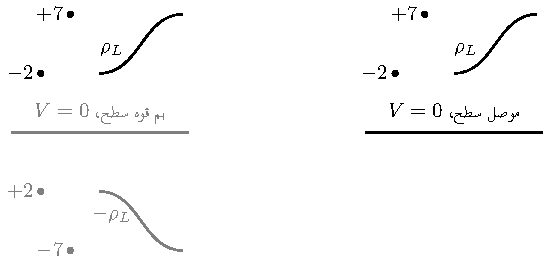
\includegraphics{figCapacitorMethodOfImages}
\caption{عکس کی ترکیب۔}
\label{شکل_کپیسٹر_عکس_کی_ترکیب}
\end{figure}

شکل  \حوالہ{شکل_کپیسٹر_عکس_کی_ترکیب} میں لامحدود موصل سطح سے اوپر مختلف اقسام کے چارج دکھائے گئے ہیں۔اسی شکل میں مسئلے کو عکس کے ترکیب کی نقطہ نظر سے بھی دکھایا گیا ہے۔موصل سطح کے مقام پر دونوں صورتوں میں صفر وولٹ ہی رہتے ہیں۔ 
%==============

\ابتدا{مثال}
 لامحدود موصل سطح \عددیء{z=3} کے قریب \عددیء{N(5,7,8)} پر \عددیء{\SI{+5}{\micro \coulomb}} چارج پایا جاتا ہے۔موصل کی سطح پر نقطہ \عددیء{M(2,4,3)} پر \عددیء{\kvec{E}} حاصل کرتے ہوئے اسی مقام پر موصل کی سطحی کثافت چارج حاصل کریں۔

حل:\عددیء{\SI{+5}{\micro \coulomb}} کا عکس \عددیء{\SI{-5}{\micro \coulomb}} لامحدود سطح کے دوسری جانب نقطہ \عددیء{P(5,7,-2)} پر رکھتے ہوئے موصل سطح ہٹاتے ہیں۔اب \عددیء{N} سے \عددیء{M} تک  سمتیہ \عددیء{\kvec{R}_{MN}=-3\ax-3\ay-5\az} ہے جبکہ \عددیء{P} سے \عددیء{M} تک  سمتیہ \عددیء{\kvec{R}_{MP}=-3\ax-3\ay+5\az} ہے۔یوں \عددیء{\SI{+5}{\micro \coulomb}} نقطہ \عددیء{M} پر 
\begin{align*}
\kvec{E}_+=\frac{5 \times 10^{-6} (-3\ax-3\ay-5\az)}{4 \pi \epsilon_0 (3^2+3^2+5^2)^{\frac{3}{2}}}=\frac{5\times 10^{-6} (-3\ax-3\ay-5\az)}{4 \pi \epsilon_0 (43)^{\frac{3}{2}}}
\end{align*}
پیدا کرے گا۔اسی طرح \عددیء{\SI{-5}{\micro \coulomb}} چارج  نقطہ \عددیء{M} پر
\begin{align*}
\kvec{E}_-=\frac{-5 \times 10^{-6}(-3\ax-3\ay+5\az)}{4 \pi \epsilon_0 (3^2+3^2+5^2)^{\frac{3}{2}}}=\frac{-5 \times 10^{-6}(-3\ax-3\ay+5\az)}{4 \pi \epsilon_0 (43)^{\frac{3}{2}}}
\end{align*}
میدان پیدا کرے گا۔چونکہ برقی میدان خطی نوعیت کا ہوتا ہے لہٰذا کسی بھی نقطے پر مختلف چارجوں کے پیدا کردہ میدان جمع کرتے ہوئے کُل میدان حاصل کیا جا سکتا ہے۔یوں نقطہ \عددیء{M} پر کُل میدان
\begin{align*}
\kvec{E}_{\textup{کل}}=\kvec{E}_+ +\kvec{E}_-=\frac{-50 \times 10^{-6} \az}{4\pi \epsilon_0 (43) ^{\frac{3}{2}}}
\end{align*}
ہو گا۔موصل کی سطح پر میدان عمودی ہوتا ہے۔موجودہ جواب اس حقیقت کی تصدیق کرتا ہے۔یوں موصل کی سطح پر 
\begin{align*}
\kvec{D}=\epsilon_0 \kvec{E}=\frac{-50\times 10^{-6} \az}{4\pi (43) ^{\frac{3}{2}}}=-14.13\times 10^{-9} \az
\end{align*}
حاصل ہوتا ہے جو سطح میں داخل ہونے کی سمت میں ہے۔یوں مساوات \حوالہ{مساوات_کپیسٹر_سرحد_موصل_خلاء_عمودی_میدان} کے تحت سطح پر 
\begin{align*}
\rho_S=-14.3  \si{\nano \coulomb \per \meter \squared}
\end{align*}
پایا جاتا ہے۔
\انتہا{مثال}
%====================

مندرجہ بالا مثال میں اگر \عددیء{N(5,7,8)} پر \عددیء{\SI{+5}{\micro\coulomb}}  پایا جاتا اور لامحدود سطح موجود نہ ہوتا تب \عددیء{M(2,4,3)} پر میدان \عددیء{\kvec{E}_+} ہوتا۔لامحدود موصل سطح کی موجودگی میں یہ قیمت تبدیل ہو کر مثال میں حاصل کی گئی \عددیء{\kvec{E}_{\textup{کل}}} ہو جاتی ہے۔درحقیقت سطح کے قریب چارج کی وجہ سے سطح پر سطحی چارج کثافت پیدا ہو جاتا ہے۔کسی بھی نقطے پر بیرونی چارج اور سطحی چارج دونوں کے میدان کا مجموعہ حقیقی میدان ہوتا ہے۔
%===================
\ابتدا{مثال}\شناخت{مثال_کپیسٹر_نقطہ_چارج_سے_لامحدود_سطح_میں_پیدا_کثافت}
لامحدود موصل سطح \عددیء{z=0} میں \عددیء{(0,0,z)} پر \عددیء{Q} نقطہ چارج سے پیدا کثافت سطحی چارج حاصل کریں۔ 

حل:اس مسئلے کو عکس کے ترکیب سے حل کرنے کی خاطر \عددیء{(0,0,-z)} پر \عددیء{-Q} چارج رکھتے ہوئے موصل سطح کو ہٹا کر حل کرتے ہیں۔ایسی صورت میں سطح کے مقام پر عمومی نقطہ \عددیء{(\rho, \phi,0)} پر \عددیء{Q} اور \عددیء{-Q} چارج
\begin{align*}
\kvec{E}_+&=\frac{Q (\rho \arho-z\az)}{4\pi \epsilon_0 (\rho^2+z^2)^{\frac{3}{2}}}\\
\kvec{E}_-&=\frac{-Q (\rho \arho+z\az)}{4\pi \epsilon_0 (\rho^2+z^2)^{\frac{3}{2}}}
\end{align*}
میدان پیدا کریں گے۔\عددیء{\kvec{D}=\epsilon_0 \kvec{E}} استعمال کرتے ہوئے  کُل 
\begin{align*}
\kvec{D}=\frac{-2Qz\az}{4\pi (\rho^2+z^2)^{\frac{3}{2}}}
\end{align*}  
حاصل ہوتا ہے جس کی سمت \عددیء{-\az} ہے جو موصل میں اوپر سے داخل ہونے کی سمت ہے۔یوں موصل سطح پر
\begin{align}\label{مساوات_کپیسٹر_لامحدود_سطح_پر_سطحی_کثافت}
\rho_S=\frac{-2Qz}{4\pi  (\rho^2+z^2)^{\frac{3}{2}}} \quad \quad \si{\coulomb \per \meter \squared}
\end{align}
پایا جائے گا۔شکل \حوالہ{شکل_کپیسٹر_لامحدود_سطح_پیدا-کثافت_چارج} میں چارج \عددیء{Q} اور موصل سطح پر \عددیء{\rho_S} دکھائے گئے ہیں۔
\begin{figure}
\centering
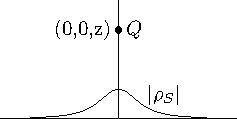
\includegraphics{figCapacitorChargeCreatedOnSurfaceDueToPointCharge}
\caption{نقطہ چارج سے لامحدود موصل سطح میں پیدا سطحی کثافت  چارج۔}
\label{شکل_کپیسٹر_لامحدود_سطح_پیدا-کثافت_چارج}
\end{figure}
\انتہا{مثال}
%======================

مساوات \حوالہ{مساوات_کپیسٹر_لامحدود_سطح_پر_سطحی_کثافت} کو استعمال کرتے ہوئے  لامحدود موصل سطح پر کل چارج حاصل کیا جا سکتا ہے۔یقینی طور پر اس کی مقدار \عددیء{-Q} ہی حاصل ہو گی۔

\حصہ{نیم موصل}
نیم موصل اشیاء مثلاً خالص سلیکان اور جرمینیم میں آزاد چارجوں کی تعداد موصل کی نسبت سے کم جبکہ غیر موصل کی نسبت سے زیادہ ہوتی ہے۔یوں ان کی موصلیت موصل اور غیر موصل کے موصلیت کے درمیان میں ہوتی ہے۔نیم موصل کی خاص بات یہ ہے کہ ان میں انتہائی کم مقدار کے \اصطلاح{ملاوٹ}\فرہنگ{ملاوٹ}\حاشیہب{doping}\فرہنگ{doping} سے ان کی موصلیت پر انتہائی گہرا اثر پڑتا ہے۔نیم موصل \اصطلاح{دوری جدول}\فرہنگ{دوری جدول}\حاشیہب{periodic table}\فرہنگ{periodic table} کے چوتھے  \اصطلاح{جماعت}\فرہنگ{جماعت}\حاشیہب{group}\فرہنگ{group} سے تعلق رکھتے ہیں۔دوری جدول کے پانچویں جماعت کے عناصر مثلاً  نائٹروجن اور فاسفورس کا ایٹم ایک عدد الیکٹران عطا کرنے کا رجحان رکھتا ہے۔یوں انہیں \اصطلاح{عطا کنندہ}\فرہنگ{عطا کنندہ}\حاشیہب{donor}\فرہنگ{donor} عناصر کہتے ہیں۔نیم موصل میں ایسا ہر عطا کنندہ ملاوٹی ایٹم ایک عدد آزاد الیکٹران کو جنم دیتا ہے۔ ایسے عنصر کی نہایت کم مقدار کی ملاوٹ سے نیم موصل میں آزاد الیکٹران کی تعداد بڑھ جاتی ہے جس سے ان کی موصلیت بہت بڑھ جاتی ہے۔ایسے نیم موصل جن میں آزاد الیکٹران کی تعداد بڑھا دی گئی ہو کو \عددیء{n} نیم موصل کہتے ہیں۔اس کے برعکس تیسرے جماعت کے عناصر مثلاً المونیم کا ایٹم ایک عدد الیکٹران قبول کرنے کا رجحان رکھتا ہے۔یوں المونیم کو \اصطلاح{قبول کنندہ}\فرہنگ{قبول کنندہ}\حاشیہب{acceptor}\فرہنگ{acceptor} عنصر کہا جاتا ہے۔ملاوٹی المونیم کا ایٹم نیم موصل کے ایٹم سے الیکٹران حاصل کرتے ہوئے  الیکٹران کی جگہ خالی جگہ پیدا کر دیتا ہے جسے \اصطلاح{خول}\فرہنگ{خول}\حاشیہب{hole}\فرہنگ{hole} کہا جاتا ہے۔نیم موصل میں ایسا ہر قبول کنندہ ملاوٹی ایٹم ایک عدد آزاد خول کو جنم دیتا ہے۔ایسا آزاد خول مثبت ذرے کی مانند معلوم ہوتا ہے جس کا چارج \عددیء{e} الیکٹران کے چارج \عددیء{-e} کے برابر مگر الٹ قطب کا ہوتا ہے اور جس کی کمیت \عددیء{m_h} لی جا سکتی ہے۔ اسی طرح آزاد خول کی حرکت پذیری \عددیء{\mu_h} لکھی جاتی ہے۔بالکل آزاد الیکٹران کی طرح برقی میدان کی موجودگی میں آزاد خول رفتار بہاو \عددیء{\kvec{v}_d=\mu_h \kvec{E}} سے حرکت کرتا ہے جو موصلیت \عددیء{\sigma=\rho_h  \mu_h}  کو جنم دیتا ہے۔یاد رہے کہ مثبت خول \عددیء{\kvec{E}} کی سمت میں ہی حرکت کرے گا لہٰذا اس کے رفتار بہاو کی سمت \عددیء{\kvec{E}} کی سمت ہی ہو گی۔تیسرے جماعت کے عناصر کی ملاوٹ کردہ نیم موصل کو \عددیء{p} نیم موصل کہا جاتا ہے۔
آزاد الیکٹران اور آزاد خول مل کر 
\begin{align}
\sigma =-\rho_e \mu_e+\rho_h \mu_h
\end{align} 
موصلیت پیدا کرتے ہیں جہاں \عددیء{\rho_h} آزاد خول کی حجمی چارج کثافت ہے۔خالص نیم موصل میں حرارتی توانائی سے نیم موصل کے ایٹم سے الیکٹران خارج ہو کر آزاد الیکٹران کی حیثیت اختیار کرتا ہے جبکہ ایسے الیکٹران کا خالی کردہ مقام آزاد خول کی حیثیت اختیار کرتا ہے۔یوں خالص نیم موصل میں آزاد الیکٹران اور آزاد خول کی تعداد برابر ہوتی ہے۔

خالص نیم موصل اوہم کے قانون کی نقطہ شکل پر پورا اترتا ہے۔یوں کسی ایک درجہ حرارت پر نیم موصل کی موصلیت تقریباً اٹل قیمت رکھتی ہے۔  

آپ کو یاد ہو گا کہ درجہ حرارت بڑھانے سے موصل میں آزاد الیکٹران کی رفتار بہاو کم ہوتی ہے جس سے موصلیت کم  ہو جاتی ہے۔درجہ حرارت کا موصل میں آزاد الیکٹران کے حجمی چارج کثافت پر خاص اثر نہیں ہوتا۔اگرچہ نیم موصل میں بھی درجہ حرارت بڑھانے سے آزاد چارج کی رفتار بہاو کم ہوتی ہے لیکن ساتھ ہی ساتھ آزاد چارج کی مقدار نسبتاً زیادہ مقدار میں بڑھتی ہے جس  کی وجہ سے نیم موصل کی  موصلیت درجہ حرارت بڑھانے سے بڑھتی ہے۔یہ موصل اور نیم موصل کے خصوصیات میں واضح فرق ہے۔
%======
\ابتدا{مشق}\شناخت{مشق_کپیسٹر_نیم_موصل_موصلیت}
\عددیء{\SI{300}{\kelvin}} درجہ حرارت پر خالص سلیکان میں آزاد الیکٹران اور آزاد خول کی تعداد \عددیء{\num{1.5e16}} فی مربع میٹر، الیکٹران کی رفتار بہاو \عددیء{\SI{0.12}{\meter \squared \per \volt  \per \second}} جبکہ خول کی رفتار بہاو \عددیء{\SI{0.025}{\meter \squared \per \volt \per \second}} ہے۔جرمینیم کے لئے یہی قیمتیں بالترتیب \عددیء{\num{2.4e19}} فی مربع میٹر، \عددیء{\SI{0.36}{\meter \squared \per \volt  \per \second}} اور \عددیء{\SI{0.17}{\meter \squared \per \volt \per \second}} ہیں۔ خالص سلیکان اور خالص جرمینیم کی موصلیت دریافت کریں۔

جوابات:\عددیء{\SI{0.348}{\milli \siemens \per \meter}} اور \عددیء{\SI{2}{\siemens \per \meter}}

\انتہا{مشق}
%===========================

\حصہ{ذو برق}
اس باب میں اب تک ہم موصل اور نیم موصل کی بات کر چکے ہیں جن میں آزاد چارج پائے جاتے ہیں۔یوں ایسے اشیاء پر برقی دباو لاگو کرنے سے ان میں برقرار برقی رو پیدا کی جا سکتی ہے۔آئیں ایسی اشیاء کی بات کریں جن میں آزاد چارج نہیں پائے جاتے لہٰذا ان میں برقرار برقی رو پیدا کرنا ممکن نہیں ہوتا۔

بعض اشیاء مثلاً پانی  کے مالیکیول میں قدرتی طور پر مثبت اور منفی مراکز پائے جاتے  ہیں۔ایسے مالیکیول کو \اصطلاح{قطبی}\فرہنگ{قطبی}\حاشیہب{polar}\فرہنگ{polar} مالیکیول کہتے ہیں۔قطبی مالیکیول کو جفت قطب\فرہنگ{جفت قطب} تصور کیا جا سکتا ہے۔بیرونی میدان کے غیر موجودگی میں کسی بھی چیز میں قطبی مالیکیول بلا ترتیب پائے جاتے ہیں۔ بیرونی میدان \عددیء{\kvec{E}} لاگو کرنے سے مالیکیول کے مثبت سرے پر میدان کی سمت میں جبکہ منفی سرے پر میدان کی الٹ سمت میں  قوت عمل کرتا ہے۔ان قوتوں کی وجہ سے مالیکیول کے مثبت اور منفی مراکز ان قوتوں کی سمتوں میں حرکت کرتے ہوئے گھوم جاتے ہیں اور ساتھ ہی ساتھ مراکز کے درمیان فاصلہ بھی بڑھ جاتا ہے۔ٹھوس قطبی اشیاء میں ایٹموں اور مالیکیول کے درمیان قوتیں ان حرکات کو روکنے کی کوشش کرتی ہیں۔اسی طرح مثبت اور منفی چارج کے مابین قوت کشش ان کے درمیان فاصلہ بڑھنے کو روکتا ہے۔جہاں یہ مخالف قوتیں برابر ہوں وہاں مثبت اور منفی مراکز رک جاتے ہیں۔بیرونی میدان ان تمام بلا ترتیب جفت قطب کو ایک سمت میں لانے کی کوشش کرتا ہے۔

بعض اشیاء میں قدرتی طور پر مثبت اور منفی مراکز نہیں پائے جاتے البتہ انہیں بیرونی میدان میں رکھنے سے ان میں ایسے مراکز پیدا ہو جاتے ہیں۔ایسے اشیاء کو \اصطلاح{غیر قطبی}\فرہنگ{غیر قطبی}\حاشیہب{non polar}\فرہنگ{non polar} کہتے ہیں۔ بیرونی میدان مالیکیول کے الیکٹرانوں کو ایک جانب کھینچ کر منفی مرکز جبکہ  بقایا ایٹم کو مثبت چھوڑ کر مثبت مرکز پیدا کرتا ہے۔مثبت اور منفی چارج کے مابین قوت کشش اس طرح مراکز پیدا ہونے کے خلاف عمل کرتا ہے۔جہاں یہ مخالف قوتیں برابر ہو جائیں وہیں پر چارج کے حرکت کا سلسلہ رک جاتا ہے۔یہ اشیاء قدرتی طور پر غیر قطبی ہیں البتہ انہیں بیرونی میدان قطبی بنا دیتا ہے۔پیدا کردہ جفت قطب بیرونی میدان کی سمت میں ہی ہوں گے۔

ایسے تمام اشیاء جو یا تو پہلے سے قطبی ہوں اور یا انہیں بیرونی میدان کی مدد سے قطبی بنایا جا سکے \اصطلاح{ذو برقی}\فرہنگ{ذو برق}\حاشیہب{dielectric}\فرہنگ{dielectric} کہلاتے ہیں۔

ذو برق میں بیرونی میدان سے مالیکیول کے اندر حرکت پیدا ہوتی ہے البتہ مالیکیول ازخود اسی جگہ رہتا ہے۔ایسا چارج جو بیرونی میدان کی وجہ سے اپنی جگہ پر معمولی حرکت کرتا ہو کو \اصطلاح{مقید چارج}\فرہنگ{چارج!مقید}\حاشیہب{bound charge}\فرہنگ{bound charge} کہتے ہیں۔ اس کے برعکس آزاد چارج بیرونی میدان میں مسلسل حرکت کرتا ہے۔ 

ذو برق کے جفت قطب کا معیار اثر کو صفحہ \حوالہصفحہ{مساوات_توانائی_سمتی_جفت_قطب} میں دئے مساوات \حوالہ{مساوات_توانائی_سمتی_جفت_قطب} 
\begin{align}
\kvec{p}=Q \kvec{d}
\end{align}
سے ظاہر کیا جا سکتا ہے جہاں \عددیء{Q} ذو برق کے جفت قطب میں مثبت مرکز کا چارج ہے۔

اگر اکائی حجم میں \عددیء{n} جفت قطب پائے جائیں تب \عددیء{\Delta v} حجم میں \عددیء{n \Delta v} جفت قطب ہوں گے جن کا اجتماعی معیار اثر جفت قطب تمام کے سمتی مجموعے
\begin{align}
\kvec{p}_{\textup{کل}}=\sum_{i=1}^{n \Delta v} \kvec{p}_i
\end{align}
 کے برابر ہو گا جہاں انفرادی \عددیء{\kvec{p}} مختلف ہو سکتے ہیں۔\اصطلاح{تقطیب}\فرہنگ{تقطیب}\حاشیہب{polarization}\فرہنگ{polarization} سے مراد اکائی حجم میں کل معیار اثر جفت قطب ہے یعنی
\begin{align}\label{مساوات_موصل_تقطیب_تعریف}
\kvec{P}=\lim_{\Delta v \to 0}\frac{1}{\Delta v} \sum_{i=1}^{n \Delta v} \kvec{p}_i
\end{align} 
جس کی اکائی کولمب فی مربع میٹر ہے۔\عددیء{\Delta v} کو کم سے کم\حاشیہد{یہ ایسے ہی ہے جیسے لمحاتی رفتار \عددیء{\tfrac{\Delta x}{\Delta t}} حاصل کرتے وقت  \عددیء{\Delta t \to 0} لیا جاتا ہے۔} کرتے ہوئے نقطے پر تقطیب حاصل کی گئی ہے۔حقیقت میں \عددیء{\Delta v} کو اتنا رکھا جاتا ہے کہ اس میں جفت قطب کی تعداد \عددیء{(n \Delta v)} اتنی ہو کہ انفرادی جفت قطب کے اثر کو نظر انداز کرنا ممکن ہو۔یوں تقطیب کو یکساں تفاعل تصور کیا جاتا ہے۔

آئیں ان حقائق کو استعمال کرتے ہوئے آگے بڑھیں۔
\begin{figure}
\centering
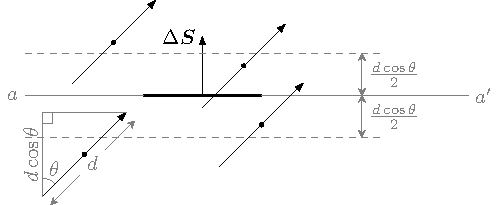
\includegraphics{figCapacitorMotionOfBoundChargesInDielectric}
\caption{بیرونی میدان کی موجودگی میں مقید چارج کی حرکت۔}
\label{شکل_کپیسٹر_مقید_چارج_حرکت}
\end{figure}

شکل  \حوالہ{شکل_کپیسٹر_مقید_چارج_حرکت} کو دیکھتے ہوئے آگے پڑھیں۔ تصور کریں کہ ذو برق میں غیر قطبی مالیکیول پائے جاتے ہیں جن کا مقام بیرونی میدان کی غیر موجودگی میں دائروں سے ظاہر کیا گیا ہے۔بیرونی میدان کے غیر موجودگی میں \عددیء{\kvec{P}=0} ہو گا۔ذو برق کے اندر تصوراتی سطح \عددیء{\Delta \kvec{S}} لیتے ہیں جسے موٹی گہری سیاہی کی لکیر سے ظاہر کیا گیا ہے۔اس کے دونوں جانب ہلکی سیاہی سے \عددیء{a} تا \عددیء{a'} لکیر بھی دکھائی گئی ہے۔بیرونی میدان لاگو کرنے سے  جفت قطب \عددیء{\kvec{p}=Q\kvec{d}} پیدا ہوتے ہیں  جن کا \عددیء{\kvec{d}} اور \عددیء{\kvec{p}} سطح  \عددیء{\Delta \kvec{S}} کے ساتھ \عددیء{\theta} زاویہ بناتے ہیں۔ان جفت قطب کو سمتیوں سے ظاہر کیا گیا ہے جہاں سمتیہ کی نوک مثبت جبکہ اس کی دم منفی چارج کا مقام دیتی ہے۔شکل کو دیکھتے ہوئے صاف ظاہر ہے  کہ \عددیء{aa'} سے \عددیء{\tfrac{d\cos \theta}{2}} فاصلے نیچے  تک تمام مثبت چارج بیرونی میدان لاگو کرنے سے  \عددیء{aa'} سے گزرتے ہوئے  اوپر چلے جائیں گے۔ اسی طرح \عددیء{aa'} سے \عددیء{\tfrac{d\cos \theta}{2}} فاصلے اوپر  تک تمام منفی چارج بیرونی میدان لاگو کرنے سے  \عددیء{aa'} سے گزرتے ہوئے  نیچے چلے جائیں گے۔یوں \عددیء{\Delta S} رقبہ اور \عددیء{d\cos \theta} گہرائی کے حجم \عددیء{d \Delta S \cos \theta} میں جتنے بھی جفت قطب ہوں ان تمام کا ایک سرا \عددیء{\Delta \kvec{S}} سے گزرے گا۔چونکہ اکائی حجم میں \عددیء{n} جفت قطب ہیں لہٰذا اتنی حجم میں \عددیء{n d \Delta S \cos \theta} جفت قطب ہوں گے۔یوں \عددیء{\tfrac{n Qd \Delta S \cos \theta}{2}} چارج \عددیء{\Delta S} سے گزر کر اوپر  جبکہ \عددیء{\tfrac{-n Qd \Delta S \cos \theta}{2}} چارج \عددیء{\Delta S} سے گزر کر نیچے جائے گا۔مثبت چارج کا اوپر جانب حرکت اور منفی چارج کا نیچے جانب حرکت ایک ہی معنی رکھتے ہیں لہٰذا  کل 
\begin{align}\label{مساوات_کپیسٹر_مقید_چارج_الف}
\Delta Q_m=nQd \Delta S \cos \theta=n Q  \kvec{d} \cdot \Delta \kvec{S}
\end{align}
چارج سطح سے گزرتے ہوئے اوپر جانب جائے گا جہاں \عددیء{\Delta Q_m} لکھتے ہوئے اس حقیقت کی یاد دہانی کرائی گئی ہے کہ ہم مقید چارج کی بات کر رہے ہیں۔چونکہ تمام جفت قطب ایک ہی سمت میں ہیں لہٰذا اس حجم کی تقطیب
\begin{align}
\kvec{P}=nQ\kvec{d}
\end{align}
ہو گی۔یوں مساوات \حوالہ{مساوات_کپیسٹر_مقید_چارج_الف} کو
\begin{align}\label{مساوات_کپیسٹر_مقید_چارج_ب}
\Delta Q_m=\kvec{P} \cdot \Delta \kvec{S}
\end{align}
لکھا جا سکتا ہے۔اگر \عددیء{\Delta \kvec{S}} کو بند سطح کا ٹکڑا سمجھا جائے جہاں \عددیء{\kvec{a}_S} بیرونی سمت کو ہو تب اس بند سطح سے کل چارج کا اخراج 
\begin{align*}
\oint_S \kvec{P} \cdot \dif \kvec{S}
\end{align*}
کے برابر ہو گا۔یوں بند سطح میں مقید چارج کا اضافہ
\begin{align}\label{مساوات_کپیسٹر_مقید_چارج}
Q_m=-\oint_S \kvec{P} \cdot \dif \kvec{S}
\end{align}
ہو گا۔یہ مساوات گاوس کے قانون کی شکل رکھتی ہے لہٰذا ہم کثافت برقی بہاو کی تعریف یوں تبدیل کرتے ہیں کہ یہ خالی خلاء کے علاوہ دیگر صورتوں میں بھی قابل استعمال ہو۔گاوس کا قانون صحہ \حوالہصفحہ{مساوات_گاوس_قانون_گاوس_بنیادی_شکل} پر مساوات \حوالہ{مساوات_گاوس_قانون_گاوس_بنیادی_شکل} میں دیا گیا ہے۔ہم پہلے اس قانون کو \عددیء{\epsilon_0\kvec{E}} اور کل گھیرے چارج \عددیء{Q_{\textup{کل}}} کی شکل میں لکھتے ہیں
\begin{align}\label{مساوات_کپیسٹر_گاوس_قانون}
Q_{\textup{کل}}=\oint_S \epsilon_0 \kvec{E} \cdot \dif \kvec{S}
\end{align}
جہاں 
\begin{align}\label{مساوات_کپیسٹر_کل_چارج}
Q_{\textup{کل}}=Q+Q_m
\end{align}
کے برابر ہے۔مساوات \حوالہ{مساوات_کپیسٹر_گاوس_قانون} میں بند سطح \عددیء{\kvec{S}} آزاد چارج \عددیء{Q} اور مقید چارج \عددیء{Q_m} کو گھیرے ہوئے ہے۔مساوات \حوالہ{مساوات_کپیسٹر_کل_چارج} میں مساوات \حوالہ{مساوات_کپیسٹر_مقید_چارج} اور مساوات \حوالہ{مساوات_کپیسٹر_گاوس_قانون} پر کرتے ہوئے
\begin{align}
Q=Q_{\textup{کل}}-Q_m=\oint_S (\epsilon_0 \kvec{E}+\kvec{P}) \cdot \dif \kvec{S}
\end{align}
حاصل ہوتا ہے۔

ہم کثافت برقی بہاو کو اب
\begin{align}\label{مساوات_کپیسٹر_برقی_بہاو_اور_تقطیب}
\kvec{D}=\epsilon_0 \kvec{E}+\kvec{P}
\end{align}
بیان کرتے ہیں جو زیادہ کارآمد اور عمومی مساوات ہے۔یوں ذو برق اشیاء کے لئے کثافت برقی بہاو میں اضافی جزو \عددیء{\kvec{P}} شامل ہو جاتا ہے۔اس طرح
\begin{align}\label{مساوات_کپیسٹر_گاوس_عمومی_مساوات}
Q=\oint_S \kvec{D} \cdot \dif \kvec{S}
\end{align}
لکھا جا سکتا ہے جہاں \عددیء{Q} گھیرا ہوا آزاد چارج ہے۔

ہم آزاد، مقید اور کُل چارجوں کے لئے آزاد، مقید اور کُل حجمی کثافت بیان کرتے ہوئے
\begin{align*}
Q&=\int_h \rho_h \dif h\\
Q_m&=\int_h \rho_m \dif h\\
Q_{\textup{کل}}&=\int_h \rho_{\textup{کل}} \dif h\\
\end{align*}
لکھ سکتے ہیں۔

مسئلہ پھیلاو کے استعمال سے مساوات \حوالہ{مساوات_کپیسٹر_مقید_چارج}، مساوات \حوالہ{مساوات_کپیسٹر_گاوس_قانون} اور مساوات \حوالہ{مساوات_کپیسٹر_گاوس_عمومی_مساوات} کے نقطہ اشکال
\begin{align*}
\nabla \cdot \kvec{P}&=-\rho_m \\
\epsilon_0 \nabla \cdot \kvec{E}&=\rho_{\textup{کل}} 
\end{align*}
اور
\begin{align}
\nabla \cdot \kvec{D}&=\rho_h
\end{align}

لکھے جا سکتے ہیں۔

قلم میں دہراتے طرز پر ایٹم پائے جاتے ہیں۔قلم میں عموماً کسی ایک سمت میں با آسانی جبکہ بقایا سمتوں میں مشکل سے تقطیب پیدا کرنا ممکن ہوتا ہے۔جس سمت میں باآسانی تقطیب پیدا کی جا سکے اسے \اصطلاح{آسان محور}\فرہنگ{آسان محور}\حاشیہب{easy axis}\فرہنگ{easy axis} یا \اصطلاح{آسان سمت}\فرہنگ{آسان سمت} یا \اصطلاح{نرم محور}\فرہنگ{نرم محور} کہتے ہیں۔۔ایسے اشیاء جو مختلف اطراف میں مختلف خصوصیات رکھتے ہوں \اصطلاح{سمتی}\فرہنگ{سمتی}\حاشیہب{anisotropic}\فرہنگ{anisotropic} اشیاء کہلاتے ہیں۔ساتھ ہی ساتھ یہ ضروری نہیں کہ بیرونی لاگو میدان اور تقطیب ایک ہی سمت میں ہوں۔کچھ ایسے اشیاء بھی پائے جاتے ہیں جو \اصطلاح{برقی چال}\فرہنگ{برقی چال}\حاشیہب{ferroelectric}\فرہنگ{ferroelectric} کی خاصیت رکھتے ہیں۔ان میں تقطیب کی قیمت ان اشیاء کی گزشتہ تاریخ پر مبنی ہوتی ہے۔یہ عمل بالکل مقناطیسی مادے کی مقناطیسی چال کے طرز کی خصوصیت ہے۔ 
   
کچھ ذو برق اشیاء میں لاگو بیرونی میدان \عددیء{\kvec{E}} اور تقطیب \عددیء{\kvec{P}} ہر صورت ایک ہی سمت میں ہوتے ہیں۔ ان اشیاء کی خصوصیات ہر طرف بالکل ایک ہی طرح ہوتی ہیں۔ایسے اشیاء \اصطلاح{غیر سمتی}\فرہنگ{غیر سمتی}\حاشیہب{isotropic}\فرہنگ{isotropic} اشیاء کہلاتے ہیں۔انجنیئرنگ میں استعمال ہونے والے  ذو برق اشیاء عموماً ایسے ہی ہوتے ہیں۔اس کتاب میں صرف انہیں پر تبصرہ کیا جائے گا۔ایسے اشیاء میں  تقطیب اور لاگو برقی میدان راست تناسب تعلق
\begin{gather}
\begin{aligned}
\kvec{P}&=\chi_e \epsilon_0 \kvec{E}\\
&=(\epsilon_R-1)\epsilon_0 \kvec{E}
\end{aligned}
\end{gather}
رکھتا ہے جہاں مساوات کے مستقل کو \عددیء{\chi_e \epsilon_0} یا \عددیء{(\epsilon_R-1)\epsilon_0} لکھا جاتا ہے۔یوں مساوات \حوالہ{مساوات_کپیسٹر_برقی_بہاو_اور_تقطیب}
\begin{align*}
\kvec{D}=\epsilon_0 \kvec{E}+(\epsilon_R-1)\epsilon_0 \kvec{E}
\end{align*}
یا
\begin{align}
\kvec{D}=\epsilon_R\epsilon_0 \kvec{E}=\epsilon \kvec{E}
\end{align}
شکل اختیار کرتا ہے جہاں ذو برق کا \اصطلاح{برقی مستقل}
\begin{align}
\epsilon=\epsilon_R \epsilon_0
\end{align}
کے برابر ہے۔ماہر طبیعیات عموماً \عددیء{\chi_e}  جبکہ انجنیئر عموماً \عددیء{\epsilon_R} استعمال کرتے ہیں۔ان کا تعلق
\begin{align}
\chi_e=\epsilon_R-1
\end{align}
ہے۔

\عددیء{\chi_e} \اصطلاح{برقی اثر پذیری}\فرہنگ{برقی!اثر پذیری}\فرہنگ{اثر پذیری!برقی}\حاشیہب{electric susceptibility}\فرہنگ{susceptibility!electric}\فرہنگ{electric!susceptibility}، \عددیء{\epsilon_R} \اصطلاح{جزوی برقی مستقل}\فرہنگ{جزوی برقی مستقل}\حاشیہب{relative electric constant, relative permittivity}\فرہنگ{electric constant!relative}\فرہنگ{permittivity!relative} جبکہ  \عددیء{\epsilon_0} \اصطلاح{خالی خلاء کا برقی مستقل}\فرہنگ{برقی مستقل!خالی خلاء}\حاشیہب{permittivity of vacuum, electric constant of vacuum}\فرہنگ{electric constant!vacuum}  کہلاتے ہیں۔ اس کتاب کے آخر میں صفحہ \حوالہصفحہ{جدول_جدول_جزوی_برقی_مستقل_زاویہ_زیاع} پر  چند مخصوص اشیاء کے برقی مستقل جدول \حوالہ{جدول_جدول_جزوی_برقی_مستقل_زاویہ_زیاع} میں دئے گئے ہیں۔

غیر یکساں\فرہنگ{یکساں!غیر}\حاشیہب{non homogeneous}\فرہنگ{non homogeneous} خاصیت رکھنے والے اشیاء اتنے سادہ مساوات سے نہیں نپٹے جاتے۔ان اشیاء میں \عددیء{\kvec{E}} کا ہر کارتیسی جزو \عددیء{\kvec{D}}   کے ہر کارتیسی جزو پر اثر انداز ہوتا ہے لہٰذا ان کا تعلق یوں
\begin{gather}
\begin{aligned}\label{مساوت_کپیسٹر_تناوی-مساوات}
D_x&=\epsilon_{xx} E_x +\epsilon_{xy} E_y+\epsilon_{xz} E_z\\
D_y&=\epsilon_{yx} E_x +\epsilon_{yy} E_y+\epsilon_{yz} E_z\\
D_z&=\epsilon_{zx} E_x +\epsilon_{zy} E_y+\epsilon_{zz} E_z
\end{aligned}
\end{gather}
لکھا جاتا ہے جہاں نو اعدادی \عددیء{\epsilon_{ij}} کو مجموعی طور پر \اصطلاح{تناوی مستقل}\فرہنگ{تناوی مستقل}\حاشیہب{tensor}\فرہنگ{tensor} کہا جاتا ہے۔اسی طرح مساوات \حوالہ{مساوت_کپیسٹر_تناوی-مساوات} کے طرز کے مساوات \اصطلاح{تناوی} مساوات کہلاتے ہیں۔غیر سمتی اشیاء میں \عددیء{\kvec{D}} اور  \عددیء{\kvec{E}} (اور \عددیء{\kvec{P}}) آپس میں متوازی نہیں  ہوتے اور اگرچہ \عددیء{\kvec{D}=\epsilon_0 \kvec{E}+\kvec{P}} ان کے لئے بھی درست ہے، \عددیء{\kvec{D}=\epsilon \kvec{E}} استعمال کرتے وقت  اس حقیقت کا خیال رکھنا ہو گا کہ \عددیء{\epsilon} اب تناوی مستقل ہے۔غیر سمتی اشیاء پر ایک مثال کے بعد بحث روکتے ہیں۔
%============

\ابتدا{مثال}
ایک غیر سمتی ذو برق کا تناوی مستقل
\begin{align*}
\epsilon=\epsilon_0 
\begin{vmatrix}
4 & 0 & 0 \\
0 & 9 & 0\\
0 & 0 &9
\end{vmatrix}
\end{align*}
ہے۔برقی میدان \عددیء{\kvec{E}=\sqrt{3} \ax}، \عددیء{\kvec{E}=\sqrt{3}\ay} اور \عددیء{\kvec{E}=1\ax+1\ay+1\az} کی صورت میں \عددیء{\kvec{D}} حاصل کریں۔

جوابات: \عددیء{\kvec{D}=4 \sqrt{3} \epsilon_0 \ax}، \عددیء{\kvec{D}=9\epsilon_0 \ay} اور \عددیء{\kvec{D}=\epsilon_0(4\ax+9\ay+9\az)}
\انتہا{مثال}
%==========================

اس مثال میں تینوں بار \عددیء{\abs{E}=\sqrt{3}} رہا جبکہ \عددیء{D} کی قیمتیں خاصی مختلف ہیں۔یہی غیر سمتی ذو برق کی پہچان ہے۔
%==========================
 
\ابتدا{مشق}
مندرجہ ذیل صورتوں میں تقطیب حاصل کریں۔ (الف) ذو برق میں \عددیء{E=\SI{5}{\kilo \volt \per \meter}} کی صورت میں \عددیء{D=\SI{1.2}{\micro \coulomb \per \meter \squared}} پایا جاتا ہے۔(ب) \عددیء{D=\SI{2}{\micro \coulomb \per \meter \squared}} اور \عددیء{\chi_e=1.5} ہیں۔ (پ)ذو برق میں  \عددیء{\num{6e20}} مالیکیول فی مربع میٹر ہیں جہاں \عددیء{E=\SI{100}{\kilo \volt \per \meter}} پر  ہر مالیکیول کا معیار جفت قطب
 \عددیء{\SI{1.2e-26}{\coulomb \meter}} ہے۔ 

جوابات: \عددیء{\SI{1.156}{\micro \coulomb \per \meter \squared}}، \عددیء{\SI{1.2}{\micro \coulomb \per \meter \squared}} اور \عددیء{\SI{7.2}{\micro \coulomb \per \meter \squared}}
\انتہا{مشق}
%====================

\حصہ{کامل ذو برق کے سرحد پر برقی شرائط}
دو مختلف ذو برق کے سرحدی برقی شرائط\فرہنگ{سرحدی شرائط!برقی میدان}\فرہنگ{برقی!سرحدی شرائط}\حاشیہب{boundary conditions}\فرہنگ{boundary conditions!electric field}\فرہنگ{electric field!boundary conditions} شکل \حوالہ{شکل_کپیسٹر_ذو_برق_سرحدی_برقی_شرائط} کی مدد سے حاصل کرتے ہیں جہاں پہلے ذو برقی کا برقی مستقل \عددیء{\epsilon_1} جبکہ دوسرے ذو برق کا برقی مستقل \عددیء{\epsilon_2} ہے۔پہلے مماسی اجزاء حاصل کرنے کی خاطر مستطیلی راستہ \عددیء{abcd} پر
\begin{align*}
\oint \kvec{E} \cdot \dif \kvec{L}=0
\end{align*}
یعنی
\begin{align*}
E_{m1} \Delta w-E_{n1,b}\frac{\Delta h}{2}-E_{n2,b} \frac{\Delta h}{2}-E_{m2}\Delta w+E_{n2,a}\frac{\Delta h}{2}+E_{n1,a} \frac{\Delta h}{2}=0 
\end{align*} 
لکھتے ہیں جس سے
\begin{align*}
(E_{m1} -E_{m2})\Delta w +(E_{n1,a}+E_{n2,a}-E_{n1,b}-E_{n2,b})\frac{\Delta h}{2}=0
\end{align*} 
حاصل ہوتا ہے۔\عددیء{\Delta w} اتنا چھوٹا لیا جاتا ہے کہ اس پر مماسی میدان کو یکساں تصور کرنا ممکن ہو۔ مستطیل کے بائیں اور دائیں اطراف کے میدان کو زیر نوشت میں \عددیء{a} اور \عددیء{b} سے ظاہر کیا گیا ہے۔سرحدی شرائط حاصل کرنے کی خاطر سطح کے قریب تر جانا ہو گا۔ایسا کرنے سے \عددیء{\Delta h \to 0} ہو گا جس سے
\begin{align*}
(E_{n1,a}+E_{n2,a}-E_{n1,b}-E_{n2,b})\frac{\Delta h}{2} \to 0
\end{align*} 
ہو کر قابل نظر انداز ہو گا۔یوں
\begin{align*}
(E_{m1} -E_{m2})\Delta w =0
\end{align*} 
رہ جاتا ہے جس سے 
\begin{align}\label{مساوات_کپیسٹر_دو_ذو_برق_سرحدی_شرائط_الف}
E_{m1} =E_{m2}
\end{align} 
حاصل ہوتا ہے جسے
\begin{align}\label{مساوات_کپیسٹر_دو_ذو_برق_سمتی_سرحدی_شرائط_الف}
\aN \times \left(\kvec{E}1-\kvec{E}_2 \right)=0
\end{align} 
بھی لکھا جا سکتا ہے۔اس مساوات سے
\begin{align*}
\frac{D_{m1}}{\epsilon_1}=E_{m1}=E_{m2}=\frac{D_{m2}}{\epsilon_2}
\end{align*}
یعنی
\begin{align}\label{مساوات_کپیسٹر_دو_ذو_برق_سرحدی_شرائط_ب}
\frac{D_{m1}}{D_{m2}}=\frac{\epsilon_1}{\epsilon_2}
\end{align}
یا
\begin{align}\label{مساوات_کپیسٹر_دو_ذو_برق_سمتی_سرحدی_شرائط_ب}
\aN \times \left(\kvec{D}_1-\frac{\epsilon_1}{\epsilon_2} \kvec{D}_2 \right)=0
\end{align}
لکھا جا سکتا ہے۔

مساوات \حوالہ{مساوات_کپیسٹر_دو_ذو_برق_سرحدی_شرائط_الف} کہتا ہے کہ ایک ذو برقی سے دوسرے ذو برق میں داخل ہوتے ہوئے سرحد پر مماسی برقی شدت \اصطلاح{بلا جوڑ}\فرہنگ{بلا جوڑ}\حاشیہب{continuous}\فرہنگ{continuous}  ہوتا ہے۔اس کے برعکس مساوات \حوالہ{مساوات_کپیسٹر_دو_ذو_برق_سرحدی_شرائط_ب} کہتا ہے کہ دو ذو برق کے سرحد پر مماسی برقی بہاو \اصطلاح{جوڑ دار}\فرہنگ{جوڑ دار}\حاشیہب{discontinuous}\فرہنگ{discontinuous} ہوتا ہے۔یوں ایک ذو برق سے دوسرے ذو برق میں داخل ہوتے  ہوئے مماسی برقی بہاو میں \اصطلاح{سیڑھی نما}\فرہنگ{سیڑھی نما}\حاشیہب{step}\فرہنگ{step} تبدیلی پائی جاتی ہے۔


\begin{figure}
\centering
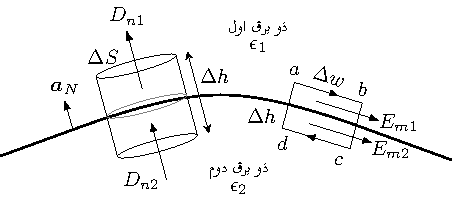
\includegraphics{figCapacitorElectricFieldDielectricDielectricBoundaryCondition}
\caption{دو مختلف ذو برق کے سرحد پر برقی شرائط۔}
\label{شکل_کپیسٹر_ذو_برق_سرحدی_برقی_شرائط}
\end{figure}

عمودی اجزاء حاصل کرنے کی خاطر گاؤس کا قانون شکل میں رقبہ \عددیء{\Delta S} گھیرتے  بیلن پر لاگو کرتے ہوئے

\begin{align}\label{مساوات_کپیسٹر_دو-ذو_برق_بیلن}
\int \limits_{\Delta S} \kvec{D}_{n1}  \cdot \dif \kvec{S} +\int \limits_{\Delta S} \kvec{D}_{n2} \cdot \dif \kvec{S} +\int \limits_{\textup{\RL{نلکی سطح}}} \kvec{D}_m \cdot \dif \kvec{S}=\int \limits_{\Delta S} \rho_S \dif S
\end{align}
لکھا جا سکتا ہے۔چھوٹے رقبہ پر میدان کو یکساں تصور کرتے ہوئے تکمل کے باہر لے جاتے ہوئے مساوات \حوالہ{مساوات_کپیسٹر_دو-ذو_برق_بیلن} کے پہلے جزو سے
\begin{align*}
\int \limits_{\Delta S} \kvec{D}_{n1}  \cdot \dif \kvec{S}=D_{n1} \Delta S
\end{align*}
حاصل ہوتا ہے۔یاد رہے کہ بند سطح کی سمت باہر کو ہوتی ہے لہٰذا \عددیء{\kvec{D}_{n1}} اور بیلن کا بالائی ڈھکن  ایک ہی سمت رکھتے ہیں جبکہ  \عددیء{\kvec{D}_{n2}} اور بیلن کا نچلا ڈھکن  الٹ سمت میں ہیں۔مساوات \حوالہ{مساوات_کپیسٹر_دو-ذو_برق_بیلن} کا دوسرا جزو
\begin{align*}
\int \limits_{\Delta S} \kvec{D}_{n2}  \cdot \dif \kvec{S}=-D_{n2} \Delta S
\end{align*}
دیتا ہے۔سطح کے قریب سے قریب ہونے سے \عددیء{\Delta h \to 0} ہو گا جس سے نلکی سطح کا رقبہ قابل نظر انداز ہو گا جس سے مساوات \حوالہ{مساوات_کپیسٹر_دو-ذو_برق_بیلن} کا تیسرا جزو صفر ہو جاتا ہے جبکہ
\begin{align*}
\int \limits_{\Delta S} \rho_S \dif S = \rho_S \Delta S
\end{align*}
کے برابر ہے۔ان تمام نتائج سے
\begin{align*}
D_{n1} \Delta S-D_{n2} \Delta S=\rho_S \Delta S
\end{align*}
یعنی
\begin{align}
D_{n1} -D_{n2} =\rho_S 
\end{align}
حاصل ہوتا ہے جسے
\begin{align}
\aN \cdot \left(\kvec{D}_1-\kvec{D}_2 \right) =\rho_S 
\end{align}
بھی لکھا جا سکتا ہے۔یوں \عددیء{D=\epsilon E} کے استعمال سے
\begin{align}
\aN \cdot \left(\epsilon_1 \kvec{E}_1-\epsilon_2 \kvec{E}_2 \right) =\rho_S 
\end{align}
حاصل ہوتا ہے۔

جزوی برقی مستقل کی مدد سے مقید چارج کا حساب رکھا جاتا ہے۔ اس طرح مقید چارج  کا علیحدہ طور پر  خیال رکھنے کی ضرورت نہیں رہتی۔یوں مندرجہ بالا مساوات میں \عددیء{\rho_S} مقید چارج نہیں ہے۔ \عددیء{\rho_S} سرحد پر با مقصد طور   رکھی گئی سطحی چارج کثافت ہے۔اس منفرد  صورت، جہاں سرحد پر از خود چارج رکھا جائے،  کے علاوہ دو ذو برق کی سرحد پر کبھی چارج نہیں پایا جاتا۔انجنیئرنگ مسائل میں عموماً \عددیء{\rho_S=0} ہی ہوتا ہے۔ایسی صورت میں مندرجہ بالا مساوات نسبتاً سادہ شکل 
\begin{align}\label{مساوات_کپیسٹر_عمودی_برقی_بہاو_مسلسل_ہے}
D_{n1} =D_{n2}
\end{align}
اختیار کر لیتی ہے جس سے
\begin{align}
\epsilon_{1} E_{n1}= D_{n1}=D_{n2}=\epsilon_2 E_{n2}
\end{align}
لکھا جا سکتا ہے۔یوں سرحد پار کرتے وقت \عددیء{E_n} میں سیڑھی نما تبدیلی پائے جاتی ہے۔اس حقیقت کو ہم یوں بیان کرتے ہیں کہ سرحد پر \عددیء{E_n} \اصطلاح{جوڑ دار}\فرہنگ{جوڑ دار}\حاشیہب{discontinuous}\فرہنگ{discontinuous} ہے۔اس کے برعکس \عددیء{D_n} سرحد پر \اصطلاح{بلا جوڑ} ہے۔

\begin{figure}
\centering
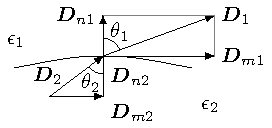
\includegraphics{figCapacitorDielectricDielectricBoundaryElectricFieldAngles}
\caption{\عددیء{\epsilon_1>\epsilon_2} کی صورت میں \عددیء{D_1>D_2} ہو گا۔اسی طرح \عددیء{\theta_1>\theta_2} جبکہ \عددیء{E_1<E_2} ہو گا۔}
\label{شکل_کپیسٹر_دو_ذو_برق_پر_بہاو}
\end{figure}
آئیں ان جوابات کی مدد سے سرحد کے دونوں جانب برقی میدان کا تعلق حاصل کریں۔شکل \حوالہ{شکل_کپیسٹر_دو_ذو_برق_پر_بہاو} کو دیکھتے ہوئے ہم 
\begin{align*}
D_{m1}&=D_1 \sin \theta_1\\
D_{n1}&=D_1 \cos \theta_1\\
D_{m2}&=D_2\sin\theta_2\\
D_{n2}&=D_2 \cos \theta_2
\end{align*}
لکھ سکتے ہیں جن سے
\begin{align*}
\frac{D_{n1}}{D_{n2}}&=\frac{D_1 \cos \theta_1}{D_2\cos\theta_2}=1 \\
\frac{D_{m1}}{D_{m2}}&=\frac{D_1 \sin \theta_1}{D_2\sin\theta_2}=\frac{\epsilon_1}{\epsilon_2}
\end{align*}
لکھا جا سکتا ہے جہاں مساوات \حوالہ{مساوات_کپیسٹر_عمودی_برقی_بہاو_مسلسل_ہے} اور  مساوات \حوالہ{مساوات_کپیسٹر_دو_ذو_برق_سرحدی_شرائط_ب} کا استعمال کیا گیا ہے۔انہیں
\begin{gather}
\begin{aligned}\label{مساوات_کپیسٹر_برقی_بہاو_سرحد_دونوں_جانب}
D_1 \cos \theta_1&=D_2 \cos \theta_2\\
\epsilon_2 D_1 \sin \theta_1&=\epsilon_1 D_2\sin\theta_2
\end{aligned}
\end{gather}
لکھ سکتے ہیں۔ان میں دوسری مساوات کو پہلی مساوات سے تقسیم کرتے ہیں
\begin{align*}
\frac{\epsilon_2 D_1 \sin \theta_1}{D_1 \cos \theta_1}&=\frac{\epsilon_1 D_2\sin\theta_2}{D_2 \cos \theta_2}
\end{align*}
جس سے
\begin{align}
\frac{\tan \theta_1}{\tan \theta_2}=\frac{\epsilon_1}{\epsilon_2}
\end{align}
حاصل ہوتا ہے۔یہ مساوات سرحد کے دونوں جانب میدان کے زاویوں کا تعلق بیان کرتا ہے۔چونکہ \عددیء{\kvec{D}=\epsilon \kvec{E}} ہوتا ہے لہٰذا سرحد کے کسی بھی طرف، اس طرف کا \عددیء{\kvec{E}} اور \عددیء{\kvec{D}} ایک ہی سمت رکھتے ہیں۔  شکل میں \عددیء{\epsilon_1 > \epsilon_2} تصور کیا گیا ہے لہٰذا اس میں \عددیء{\theta_1 > \theta_2} ہے۔

مساوات \حوالہ{مساوات_کپیسٹر_برقی_بہاو_سرحد_دونوں_جانب} کے پہلے جزو کا مربع لیتے ہوئے
\begin{align*}
D_1^2 \cos^2 \theta_1&=D_2^2 \cos^2 \theta_2\\
&=D_2^2 (1-\sin^2 \theta_2)\\
&=D_2^2-D_2^2 \sin^2\theta_2
\end{align*}
اس میں مساوات \حوالہ{مساوات_کپیسٹر_برقی_بہاو_سرحد_دونوں_جانب} کے دوسرے جزو سے \عددیء{D_2 \sin \theta_2} کی قیمت پر کرتے ہوئے
\begin{align*}
D_1^2 \cos^2\theta_1=D_2^2-D_1^2 \left(\frac{\epsilon_2}{\epsilon_1}\right)^2\sin^2\theta_1
\end{align*}
حاصل ہوتا ہے جس سے
\begin{align}
D_2=D_1\sqrt{\cos^2\theta_1+\left(\frac{\epsilon_2}{\epsilon_1}\right)^2\sin^2\theta_1}
\end{align}
ملتا ہے۔چونکہ \عددیء{E=\tfrac{D}{\epsilon}} ہے لہٰذا مندرجہ بالا مساوات سے
\begin{align*}
E_2=\frac{D_2}{\epsilon_2}&=\frac{D_1}{\epsilon_2}\sqrt{\cos^2\theta_1+\left(\frac{\epsilon_2}{\epsilon_1}\right)^2\sin^2\theta_1}\\
&=\frac{\epsilon_1 E_1}{\epsilon_2}\sqrt{\cos^2\theta_1+\left(\frac{\epsilon_2}{\epsilon_1}\right)^2\sin^2\theta_1}
\end{align*}
یعنی
\begin{align}
E_2&=E_1\sqrt{\left(\frac{\epsilon_1}{\epsilon_2} \right)^2\cos^2\theta_1+\sin^2\theta_1}
\end{align}
حاصل ہوتا ہے۔

جس جانب برقی مستقل کی قیمت  زیادہ ہو، سرحد کے اسی طرف \عددیء{D} کی قیمت بھی زیادہ ہوتی ہے ماسوائے جب \عددیء{\theta_1=\theta_2=0} ہوں جس صورت میں  \عددیء{D_2=D_1} ہوتا ہے۔اسی طرح کم \عددیء{\epsilon} جانب \عددیء{E} کی قیمت زیادہ ہوتی ہے ماسوائے جب \عددیء{\theta_1=\theta_2=90} ہوں جس صورت میں \عددیء{E_2=E_1} ہوتا ہے۔

\حصہ{موصل اور ذو برقی کے سرحدی شرائط}\فرہنگ{سرحدی شرائط!برقی میدان}\فرہنگ{boundary conditions!electric field}
موصل اور ذو برق کے سرحد پر صورت حال تقریباً ویسے ہی ہے جیسے موصل اور خالی خلاء کے سرحد پر تھی۔موصل میں \عددیء{\kvec{E}=0} ہونے کی وجہ سے سرحد پر مستطیلی راستے پر کرچاف کے قانون سے ذو برق میں \عددیء{E_m=0} حاصل ہوتا ہے۔اس طرح \عددیء{D_m=\tfrac{E_m}{\epsilon}=0} ہو گا۔

اسی طرح سرحد پر چھوٹا بیلن \عددیء{\rho_S \Delta S} چارج کو گھیرے گا جو گاوس کے قانون کی مدد سے بیلن کے ذو برق جانب ڈھکن پر  عمودی بہاو \عددیء{D_n \Delta S} پیدا کرے گا۔یوں \عددیء{D_n=\rho_S} حاصل ہوتا ہے جس سے \عددیء{E_n=\tfrac{D_n}{\epsilon}=\tfrac{\rho_S}{\epsilon}} حاصل ہوتا ہے۔

ان نتائج سے صاف  ظاہر ہے کہ موصل اور ذو برق کے سرحد پر برقی میدان کے جوابات موصل اور خالی خلاء کے سرحد کے جوابات میں \عددیء{\epsilon_0} کی جگہ \عددیء{\epsilon} پر کرنے سے حاصل ہوتے ہیں یعنی
\begin{gather}
\begin{aligned}
D_m&=E_m=0\\
D_n&=\epsilon E_n=\rho_S
\end{aligned}
\end{gather}



\حصہ{کپیسٹر}
شکل \حوالہ{شکل_کپیسٹر_کپیسٹنس_کی_تعریف} میں دو عدد موصل \عددیء{M_1} اور \عددیء{M_2}  دکھائے گئے ہیں جن کے گرد ذو برق پایا جاتا ہے۔\عددیء{M_1} پر کل \عددیء{-Q} اور \عددیء{M_2} پر کل \عددیء{+Q} چارج پایا جاتا ہے۔ان چارجوں کے علاوہ پورے نظام میں کوئی اور چارج نہیں پایا جاتا۔یوں پورا نظام غیر چارج شدہ ہے۔چونکہ موصل پر صرف سطحی چارج پایا جاتا ہے لہٰذا دونوں موصل پر چارج سطحی چارج کثافت کی صورت میں پایا جائے گا۔

\begin{figure}
\centering
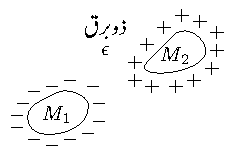
\includegraphics{figCapacitorCapacitanceDefined}
\caption{کپیسٹنس کی تعریف۔}
\label{شکل_کپیسٹر_کپیسٹنس_کی_تعریف}
\end{figure}

گاوس کے قانون کے تحت \عددیء{M_2} سے عمودی سمت میں \عددیء{+Q} کے برابر برقی بہاو کا اخراج  اور  \عددیء{M_1} پر عمودی سمت میں اتنی ہی برقی بہاو کا دخول ہو گا۔یوں موصل کے گرد ذو برق میں کثافت برقی بہاو \عددیء{\kvec{D}} اور برقی میدان کی شدت \عددیء{\kvec{E}} پائی جائے گی۔\عددیء{\kvec{D}} اور \عددیء{\kvec{E}} کی ابتدا \عددیء{M_2} سے ہو گی اور ان کا اختتام \عددیء{M_1} پر ہو گا۔

اس برقی میدان میں  کسی بھی راستے  ایک کولمب کا چارج \عددیء{M_1} تا \عددیء{M_2} منتقل کرنے کی خاطر \عددیء{V_0} توانائی درکار ہو گی۔موصل کی سطح ہم قوہ سطح ہوتی ہے لہٰذا پہلے موصل کی سطح سے کسی بھی نقطے سے دوسرے  موصل کی سطح پر کسی بھی نقطے تک چارج منتقل کرنے کی خاطر برابر توانائی درکار ہوتی ہے۔

\اصطلاح{کپیسٹنس}\فرہنگ{کپیسٹنس}\حاشیہب{capacitance}\فرہنگ{capacitance} \عددیء{C} کی تعریف
\begin{align}
C=\frac{Q}{V_0}
\end{align}
ہے جہاں \عددیء{M_1} کو صفر برقی دباو پر تصور کرتے ہوئے \عددیء{M_2} کی برقی دباو \عددیء{V_0} اور  مثبت موصل یعنی \عددیء{M_2} کا چارج \عددیء{Q} ہے۔منفی موصل سے مثبت موصل تک اکائی مثبت چارج منتقل کرنے کے لئے درکار توانائی \عددیء{V_0} کو تکمل کے ذریعے حاصل کیا جاتا ہے۔اسی طرح مثبت موصل پر چارج  \عددیء{Q} کو گاوس کے قانون کی مدد سے بذریعہ سطحی تکمل  حاصل  کیا جاتا ہے۔یوں صفحہ \حوالہصفحہ{مساوات_گاوس_قانون_گاوس_بنیادی_شکل} پر مساوات \حوالہ{مساوات_گاوس_قانون_گاوس_بنیادی_شکل} اور صفحہ \حوالہصفحہ{مساوات_توانائی_برقی_دباو_تعریف} پر مساوات \حوالہ{مساوات_توانائی_برقی_دباو_تعریف} کی مدد سے کپیسٹنس کی عمومی مساوات
\begin{align}
C=\frac{\oint_S  \epsilon \kvec{E} \cdot \dif \kvec{S} }{-\int_{-}^{+} \kvec{E} \cdot \dif \kvec{L}}
\end{align}
لکھی جا سکتی ہے۔

دونوں موصل پر چارج دگنا کرنے سے گاوس کے قانون کے تحت برقی بہاو بھی دگنی ہو جائے گی۔یوں \عددیء{\kvec{D}} اور \عددیء{\kvec{E}} بھی دگنے ہوں گے جس سے دونوں موصل کے مابین برقی دباو بھی دگنا ہو گا۔اس طرح دگنا چارج تقسیم دگنا دباو ایک بار پھر وہی کپیسٹنس دے گا۔ آپ دیکھ سکتے ہیں کہ کپیسٹنس کی قیمت کا دارومدار موصل کے اشکال، ان کے درمیان فاصلہ اور برقی مستقل پر منحصر ہے نا کہ موصل پر کل چارج کے۔

کپیسٹنس کی اکائی \اصطلاح{فیراڈ}\فرہنگ{فیراڈ}\حاشیہب{Farad}\فرہنگ{Farad} ہے جسے \عددیء{\si{\farad}} سے ظاہر کیا جاتا ہے۔ایک کولمب فی وولٹ ایک فیراڈ\حاشیہد{یہ اکائی انگلستانی ماہر طبیعیات مائکل فیراڈے کے نام سے منسوب ہے۔} کے برابر ہے۔ایک فیراڈ نہایت بڑی قیمت ہے اور عام طور کپیسٹنس کو مائیکرو فیراڈ \عددیء{\si{\micro \farad}} یا پیکو فیراڈ \عددیء{\pico \farad} میں ناپا جاتا ہے۔

\begin{figure}
\centering
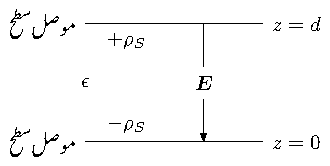
\includegraphics{figCapacitorParallelCapacitance}
\caption{متوازی چادر کپیسٹر۔}
\label{شکل_کپیسٹر_متوازی_چادر_کپیسٹر}
\end{figure}

\جزوحصہ{متوازی چادر کپیسٹر}
شکل \حوالہ{شکل_کپیسٹر_متوازی_چادر_کپیسٹر} میں دو لامحدود متوازی موصل چادر دکھائے گئے ہیں۔نچلی چادر  \عددیء{z=0} پر ہے اور اس پر سطحی چارج کثافت \عددیء{-\rho_S} پائی جاتی ہے جبکہ بالائی چادر \عددیء{z=d} پر ہے اور اس پر سطحی چارج کثافت \عددیء{+\rho_S} پائی جاتی ہے۔اس مسئلے کو ہم پہلے تفصیلی طور پر دیکھ چکے ہیں۔دو چادروں کے درمیان میدان صفحہ \حوالہصفحہ{مساوات_کولمب_متوازی_چادر_کپیسٹر_کا_میدان} پر مساوات \حوالہ{مساوات_کولمب_متوازی_چادر_کپیسٹر_کا_میدان} دیتا ہے جہاں مثبت
 چادر \عددیء{x=0} اور منفی چادر \عددیء{x=x_1} پر رکھے گئے تھے۔یوں موجودہ شکل کے مطابق مساوات \حوالہ{مساوات_کولمب_متوازی_چادر_کپیسٹر_کا_میدان} کی صورت
\begin{align*}
\kvec{E}=-\frac{\rho_S}{\epsilon} \az
\end{align*}
ہو گی۔میدان مثبت سے منفی چادر کی سمت میں ہے۔مثبت سطح سے خارج برقی بہاو کی کثافت مثبت ہے یعنی اس سطح پر عمودی \عددیء{D_+=\rho_S} کے برابر ہے جبکہ منفی چادر پر برقی بہاو داخل ہوتا ہے لہٰذا یہاں \عددیء{D_-=-\rho_S} ہو گا۔

منفی چادر کو برقی زمین تصور کرتے ہوئے مثبت چادر پر
\begin{align*}
V=-\int_0^d \kvec{E} \cdot \dif \kvec{L}=\int_0^d \frac{\rho_S \az}{\epsilon} \cdot \dif \kvec{z} \az=\int_0^d \frac{\rho_S }{\epsilon}  \dif \kvec{z}=\frac{\rho_S d}{\epsilon}
\end{align*}
برقی دباو ہو گا۔لامحدود چادر پر لامحدود چارج پایا جائے گا جس سے چادر لامحدود کپیسٹنس کا حامل ہو گا۔حقیقی کپیسٹر محدود رقبے کے چادر سے بنائے جاتے ہیں۔اگر محدود رقبے کے متوازی چادروں کے اطراف کی لمبائیاں سطحوں کے مابین فاصلے سے زیادہ ہو تو ایسی صورت میں چادروں کے درمیانی خطے میں برقی میدان  لامحدود چادروں کے میدان کی مانند ہی ہو گا۔ \عددیء{S} رقبے کے چادروں کے کپیسٹر کو لیتے ہوئے ہم دیکھتے ہیں کہ مثبت چادر پر کل
\begin{align*}
Q=\int_S \rho_S \dif S=\rho_S S
\end{align*}
چارج پایا جائے  گا۔یوں اس کی کپیسٹنس
\begin{align}\label{مساوات_کپیسٹر_دو_چادر_کپیسٹر}
C=\frac{Q}{V}=\frac{\epsilon S}{d}
\end{align}
ہو گی۔کپیسٹر کے کناروں کے قریب میدان پھول کر کپیسٹر سے باہر نکلے گا۔میدان کے \اصطلاح{پھولنے}\فرہنگ{پھولنا}\حاشیہب{fringing}\فرہنگ{fringing} کو ہم نے نظرانداز کیا ہے۔کپیسٹنس کی قیمت رقبہ بڑھا کر اور چادروں کے درمیان فاصلہ کم کرتے ہوئے حاصل کیا جاتا ہے۔اسی طرح چادروں کے درمیان زیادہ سے زیادہ برقی مستقل کا ذو برق استعمال کرتے ہوئے کپیسٹنس بڑھائی جا سکتی ہے۔

بلند تر تعدد پر چلنے والے کپیسٹر ابرق استعمال کرتے ہوئے بنائے جاتے ہیں۔\اصطلاح{ابرق کپیسٹر}\فرہنگ{کپیسٹر!ابرق}\حاشیہب{mica capacitor}\فرہنگ{capacitor!mica} انتہائی کم برقی طاقت ضائع کرتا ہے۔ابرق کی پتری کے دونوں جانب موصل مادے کی تہہ \اصطلاح{چڑھا}\فرہنگ{چڑھا}\حاشیہب{deposit}\فرہنگ{deposit} کر کپیسٹر تیار کیا جاتا ہے۔
%==================
\ابتدا{مثال}
ایک ملی میٹر کے ایک چوتھائی موٹا اور ایک سنٹی میٹر اطراف کے مربع ابرق کے پتری کے دونوں جانب المونیم کی تہہ چڑھا کر کپیسٹر تیار کیا گیا۔اس کی کپیسٹنس دریافت کریں۔

حل:کتاب کے آخر میں جدول \حوالہ{جدول_جدول_جزوی_برقی_مستقل_زاویہ_زیاع} سے ابرق کا جزوی برقی مستقل \عددیء{\epsilon_R=5.4} حاصل ہوتا ہے۔یوں
\begin{align*}
C=\frac{5.4 \times 0.01^2}{36 \pi \times 10^9 \times 0.25 \times 10^{-3}}=\SI{19.1}{\pico \farad}
\end{align*}
حاصل ہوتا ہے۔
\انتہا{مثال}
%==============================

\جزوحصہ{ہم محوری کپیسٹر}
صفحہ \حوالہصفحہ{مساوات_توانائی_ہم_محوری_تار_برقی_دباو} پر مساوات \حوالہ{مساوات_توانائی_ہم_محوری_تار_برقی_دباو} 
\begin{align*}
V=\frac{\rho_L}{2\pi\epsilon} \ln \frac{\rho_2}{\rho_1}
\end{align*}
ہم محوری تار کے دو تاروں کے درمیان برقی دباو دیتا ہے جہاں اندرونی تار پر لکیری چارج کثافت \عددیء{\rho_L} ہے۔بیرونی تار کو برقی زمین تصور کیا گیا ہے۔\عددیء{L} لمبائی کے ہم محوری تار  کے اندرونی تار پر یوں \عددیء{Q=\rho_L L} چارج پایا جائے گا۔اس طرح اتنی تار کا کپیسٹنس
\begin{align}\label{مساوات_کپیسٹر_کپیسٹر_ہم_محوری_تار}
C=\frac{Q}{V}=\frac{\rho_L L}{\frac{\rho_L}{2\pi\epsilon} \ln \frac{\rho_2}{\rho_1}}=\frac{2\pi\epsilon L}{\ln \frac{\rho_2}{\rho_1}}
\end{align}
ہو گا جہاں اندرونی تار کا رداس \عددیء{\rho_1} جبکہ بیرونی تار کا رداس \عددیء{\rho_2} ہے۔

\جزوحصہ{ہم کوہ  کپیسٹر}
محدد کے مرکز پر  \عددیء{r_A} اور \عددیء{r_B} رداس کے موصل کرہ سطح ہیں جہاں \عددیء{r_B > r_A} ہے۔اندرونی سطح پر \عددیء{+Q} اور بیرونی سطح پر \عددیء{-Q} چارج پایا جاتا ہے۔گاوس کے قانون کے تحت اندرونی سطح کے اندر یعنی \عددیء{r<r_A} اور بیرونی سطح باہر یعنی \عددیء{r>r_B} پر میدان صفر ہو گا۔دونوں سطحوں کے درمیان میدان بالکل ایسا ہی ہو گا جیسے محدد کے مرکز پر نقطہ چارج \عددیء{+Q} کا میدان ہوتا ہے۔یوں بیرونی سطح کو برقی زمین تصور کرتے ہوئے اندرونی سطح پر برقی دباو صفحہ \حوالہصفحہ{مساوات_توانائی_نقطہ_چارج_کی_دباو} پر مساوات \حوالہ{مساوات_توانائی_نقطہ_چارج_کی_دباو}
\begin{align*}
V_{AB}=\frac{Q}{4\pi \epsilon_0} \left( \frac{1}{r_A}-\frac{1}{r_B} \right)
\end{align*}
سے حاصل کیا جا سکتا ہے۔اس طرح ان سطحوں کا کپیسٹنس
\begin{align}
C=\frac{Q}{V_{AB}}=\frac{4\pi\epsilon}{\frac{1}{r_A}-\frac{1}{r_B}}
\end{align}
ہو گا۔

ایک دلچسپ صورت حال کو دیکھتے ہیں۔اگر \عددیء{r_B} کو لامحدود کر دیا جائے تب مندرجہ بالا مساوات سے
\begin{align}
C=4\pi\epsilon R \quad \quad \textup{\RL{کرہ کی کپیسٹنس}}
\end{align}
حاصل ہوتا ہے جہاں \عددیء{r_A} کی جگہ \عددیء{R} لکھا گیا ہے۔یہ مساوات رداس \عددیء{R} کرہ کی کپیسٹنس دیتا ہے۔یاد رہے کہ اس کپیسٹر کی دوسری سطح لامحدود فاصلے پر ہے۔

%================================
\ابتدا{مثال}
آپ نے بچپن میں بلور تو کھیلیں ہوں گے۔بلور کا قطر تقریباً ایک سنٹی میٹر ہوتا ہے۔خالی خلاء میں موصل بلور کی کپیسٹنس حاصل کریں۔

حل: 
\begin{align*}
C=\frac{0.5 \times 10^{-2}}{9 \times 10^9}=\SI{0.55}{\pico \farad}
\end{align*}
\انتہا{مثال}
%==============================

\عددیء{r_A} رداس کے چارج بردار موصل بلور کے اوپر \عددیء{r_A} تا \عددیء{r_1} برقی مستقل \عددیء{\epsilon_1} کے ذو برق کی تہہ چھڑانے سے \عددیء{\kvec{D}=\frac{Q}{4\pi r^2} \ar} کی بدولت
\begin{align*}
\kvec{E}=
\begin{cases}
\frac{Q}{4\pi\epsilon_1 r^2}\ar  \quad \quad (r_A < r < r_1) \\
\frac{Q}{4\pi\epsilon_0 r^2}\ar \quad \quad  (r >r_1)
\end{cases}
\end{align*}
ہو گا۔برقی زمین کو لامحدود فاصلے پر رکھتے ہوئے بلور کا برقی دباو
\begin{align*}
V&=-\int_{\infty}^{r_1}\frac{Q \dif r}{4\pi\epsilon_1 r^2} -\int_{r_1}^{r_A}\frac{Q \dif r}{4\pi\epsilon_1 r^2}\\
&=\frac{Q}{4\pi\epsilon_0 r_1} +\frac{Q}{4\pi\epsilon_1} \left(\frac{1}{r_A}-\frac{1}{r_1} \right)
\end{align*}
ہو گا جس سے کپیسٹنس
\begin{align}
C=\frac{Q}{V}=\frac{4\pi}{\frac{1}{\epsilon_0 r_1}+\frac{1}{\epsilon_1} \left(\frac{1}{r_A}-\frac{1}{r_1} \right)}
\end{align}
حاصل ہوتی ہے۔

\حصہ{سلسلہ وار اور متوازی جڑے کپیسٹر}
متوازی چادر کپیسٹر میں دو مختلف ذو برق بھرنے کا کپیسٹنس پر اثر دیکھتے ہیں۔ایسا کپیسٹر شکل \حوالہ{شکل_کپیسٹر_سلسلہ_وار} میں دکھایا گیا ہے۔چادروں کے درمیان فاصلہ چادر کے اطراف کی لمبائیوں سے نہایت کم ہونے کی صورت میں انہیں لامحدود چادروں کی طرح تصور کیا جا سکتا ہے۔منفی چادر پر \عددیء{\epsilon_1} برقی مستقل کی \عددیء{d_1} موٹائی کی تہہ  اور مثبت چادر پر \عددیء{\epsilon_2} برقی مستقل کی \عددیء{d_2} موٹائی کی تہہ ہیں۔نفی چادر پر \عددیء{-\rho_S} جبکہ مثبت چادر پر \عددیء{+\rho_S} سطحی چارج کثافت کی صورت میں چادروں کے درمیان \عددیء{D=\rho_S} ہو گا۔یوں \عددیء{\epsilon_1} ذو برق کے خطے میں
\begin{figure}[!ht]
\centering
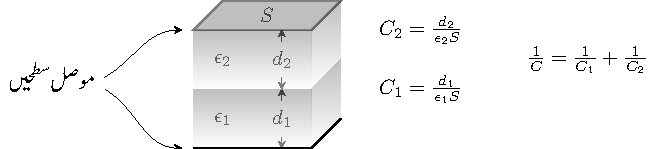
\includegraphics{figCapacitorParallelCapacitanceSeries}
\caption{سلسلہ وار کپیسٹر۔}
\label{شکل_کپیسٹر_سلسلہ_وار}
\end{figure}
%
\begin{align*}
E_1=\frac{\rho_S}{\epsilon_1}
\end{align*}
جبکہ \عددیء{\epsilon_2} ذو برق کے خطے میں
\begin{align*}
E_2=\frac{\rho_S}{\epsilon_2}
\end{align*}
لکھا جا سکتا ہے۔اس طرح 
\begin{align*}
V=E_1 d_1+E_2 d_2=\frac{\rho_S d_1}{\epsilon_1}+\frac{\rho_S d_2}{\epsilon_2}
\end{align*}
ہو گا جبکہ مثبت چادر پر چارج \عددیء{Q=\rho_S S} ہو گا جس سے کپیسٹنس
\begin{align*}
C=\frac{Q}{V}=\frac{S}{\frac{d_1}{\epsilon_1}+\frac{d_2}{\epsilon_2}}=\frac{1}{\frac{d_1}{\epsilon_1 S }+\frac{d_2}{\epsilon_2 S }}=\frac{1}{\frac{1}{C_1}+\frac{1}{C_2}}
\end{align*}
یعنی
\begin{align}
\frac{1}{C}=\frac{1}{C_1}+\frac{1}{C_2}
\end{align}
لکھی جا سکتی ہے جہاں
\begin{gather}
\begin{aligned}
C_1&=\frac{d_1}{\epsilon_1 S}\\
C_2&=\frac{d_2}{\epsilon_2 S}
\end{aligned}
\end{gather}
کے برابر ہیں۔یہی جواب شکل \حوالہ{شکل_کپیسٹر_سلسلہ_وار} میں سلسلہ وار جڑے  \عددیء{C_1} اور \عددیء{C_2} کی نشاندہی کرتے ہوئے لکھا جا سکتا ہے۔

آپ دیکھ سکتے ہیں کہ موصل متوازی دو چادروں کے درمیان تیسرے اور چوتھے ذو برق کے تہہ دئے جا سکتے ہیں۔انہیں سلسلہ وار کپیسٹر تصور کرتے ہوئے حل کیا جا سکتا ہے۔

\begin{figure}[!ht]
\centering
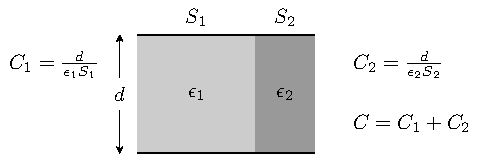
\includegraphics{figCapacitorParallelCapacitanceParallel}
\caption{متوازی جڑے کپیسٹر۔}
\label{شکل_کپیسٹر_متوازی_جڑے}
\end{figure} 

شکل \حوالہ{شکل_کپیسٹر_متوازی_جڑے} میں دو چادروں کے درمیان دو مختلف ذو برق اس طرح بھرے گئے ہیں کہ یہ متوازی جڑے کپیسٹر کو جنم دیں۔ہم شکل کو دیکھ کر ہی 
\begin{align}
C=C_1+C_2
\end{align}
لکھ سکتے ہیں۔آئیں اتنی جلدی کرنے کی بجائے اس مسئلے کا ریاضیاتی حل نکالیں۔دونوں موصل چادر ہم قوہ ہیں لہٰذا نچلی چادر کو برقی زمین یعنی صفر وولٹ اور دوسری چادر کو \عددیء{V_0} برقی دباو پر تصور کرتے ہوئے آگے بڑھتے ہیں۔یوں چادروں کے درمیان خطے میں \عددیء{E=\tfrac{V_0}{d}} ہو گا جس سے بائیں ہاتھ، یعنی \عددیء{\epsilon_1} برقہ مستقل کے ذو برق میں \عددیء{D_1=\epsilon_1 E} جبکہ دائیں ہاتھ کے ذو برق میں \عددیء{D_2=\epsilon_2 E} ہوں گے۔\عددیء{D_1} اور \عددیء{D_2} موصل چادروں کے عمودی ہیں لہٰذا سرحدی شرائط کے تحت مثبت چادر کے \عددیء{S_1} حصے پر \عددیء{\rho_{1}=D_1} جبکہ اس کے \عددیء{S_2} حصے پر \عددیء{\rho_2=D_2} ہو گا۔یوں مثبت چادر پر کل چارج
\begin{align*}
Q=\rho_1 S_1+\rho_2 S_2=\epsilon_1 \frac{V_0}{d} S_1+\epsilon_2 \frac{V_0}{d}S_2
\end{align*}
سے کپیسٹنس
\begin{align*}
C=\frac{Q}{V_0}=\frac{\epsilon_1 S_1}{d}+\frac{\epsilon_2 S_2}{d}
\end{align*}
یعنی
\begin{align}
C=C_1+C_2
\end{align}
لکھا جا سکتا ہے جہاں
\begin{gather}
\begin{aligned}
C_1&=\frac{\epsilon_1 S_1}{d}\\
C_2&=\frac{\epsilon_2 S_2}{d}
\end{aligned}
\end{gather}
کے برابر ہیں۔

\حصہ{دو متوازی تاروں کا کپیسٹنس}
شکل \حوالہ{شکل_کپیسٹر_متوازی_تار} میں دو لامحدود لمبائی کے تار \عددیء{z} محدد کے متوازی دکھائے گئے ہیں۔ہم ایسے متوازی جوڑی کی کپیسٹنس حاصل کرنا چاہتے ہیں۔ہم قوہ تار کی طرح دو متوازی تار بھی انتہائی اہم ہیں اور ان سے زندگی میں بار بار واسطہ پڑتا ہے۔
\begin{figure}
\centering
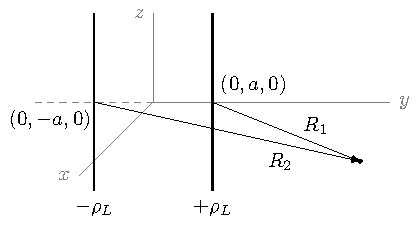
\includegraphics{figCapacitorTwoParallelWires}
\caption{دو متوازی تاروں کی کپیسٹنس۔}
\label{شکل_کپیسٹر_متوازی_تار}
\end{figure}

ایک تار جو \عددیء{(0,a,0)} سے گزرتی ہے  پر مثبت لکیری چارج کثافت \عددیء{+\rho_L} پایا جاتا ہے جبکہ دوسری تار جو \عددیء{(0,-a,0)} سے گزرتی ہے  پر منفی لکیری چارج کثافت \عددیء{-\rho_L} پایا جاتا ہے۔\عددیء{z} محدد پر لامحدود لمبائی کے لکیری چارج کثافت سے پیدا برقی دباو صفحہ \حوالہصفحہ{مساوات_توانائی_لکیری_چارج_برقی_دباو} پر مساوات \حوالہ{مساوات_توانائی_لکیری_چارج_برقی_دباو}
\begin{align*}
V=\frac{\rho_L}{2\pi \epsilon_0} \ln \frac{\rho_0}{\rho_1}
\end{align*}
 دیتا ہے جہاں برقی میدان کو \عددیء{\rho_0} پر تصور کیا گیا۔اس مساوات کو شکل \حوالہ{شکل_کپیسٹر_متوازی_تار} کے لئے ترتیب دیتے ہوئے دونوں تاروں کا مجموعی برقی دباو
\begin{align*}
V=\frac{\rho_L}{2\pi \epsilon_0}\left( \ln \frac{R_{10}}{R_1}-\ln \frac{R_{20}}{R_2} \right)=\frac{\rho_L}{2\pi \epsilon_0} \ln \frac{R_{10} R_2}{R_{20}R_1}
\end{align*}
لکھا جا سکتا ہے۔اگر \عددیء{R_{10}=R_{20}} رکھا جائے تب مندرجہ بالا مساوات 
\begin{align*}
V=\frac{\rho_L}{2\pi \epsilon_0} \ln \frac{R_2}{R_1}
\end{align*}
صورت اختیار کر لے گی۔ سطح \عددیء{y=0} پر \عددیء{R_{10}=R_{20}} ہو گا لہٰذا دراصل ہم برقی زمین کو \عددیء{y=0} سطح پر رکھ رہے ہیں۔اب \عددیء{R_1} اور \عددیء{R_2} کو \عددیء{x} اور \عددیء{y} کی صورت
\begin{align*}
\kvec{R}_1&=x\ax+(y-a)\ay\\
\kvec{R}_2&=x\ax+(y+a)\ay
\end{align*}
 میں لکھتے ہوئے
\begin{align}\label{مساوات_کپیسٹر_ہم_قوہ_سطح_کارتیسی_مساوات}
V=\frac{\rho_L}{2\pi \epsilon_0} \ln \sqrt {\frac{x^2+(y+a)^2}{x^2+(y-a)^2}}=\frac{\rho_L}{4\pi \epsilon_0} \ln \frac{x^2+(y+a)^2}{x^2+(y-a)^2}
\end{align}
یا
\begin{align}
e^{\frac{4\pi\epsilon_0 V}{\rho_L}}=\frac{x^2+(y+a)^2}{x^2+(y-a)^2}
\end{align}
لکھا جا سکتا ہے۔

ہم قوہ سطحیں حاصل کرنے کی خاطر مندرجہ بالا مساوات کو کسی اٹل برقی دباو مثلاً \عددیء{V_1} کے لئے لکھ کر حل کرتے ہیں۔چونکہ \عددیء{V_1} اٹل یا مستقل قیمت ہے جو تبدیل نہیں ہوتا لہٰذا مندرجہ بالا مساوات میں
\begin{align}\label{مساوات_کپیسٹر_زمین_موٹی_تار_جزوی_مستقل}
K_1=e^{\frac{4\pi\epsilon_0 V_1}{\rho_L}}
\end{align}
لکھ کر اسے 
\begin{align*}
K_1=\frac{x^2+(y+a)^2}{x^2+(y-a)^2}
\end{align*}
لکھا جا سکتا ہے جسے حل کرتے ہوئے
\begin{align*}
x^2+y^2-2ay \frac{K_1+1}{K_1-1} =-a^2
\end{align*}
لکھا جا سکتا ہے۔مساوات کے دونوں جانب \عددیء{a^2\tfrac{(K_1+1)^2}{(K_1-1)^2}} جمع کرتے ہوئے یوں
\begin{align}\label{مساوات_کپیسٹر_دو_تار_کپیسٹر_بنیادی}
x^2+\left[y-a\left(\frac{K_1+1}{K_1-1}\right) \right]^2=\left(\frac{2a\sqrt{K_1}}{K_1-1} \right)^2
\end{align}
لکھا جا سکتا ہے جو رداس \عددیء{\tfrac{2a\sqrt{K_1}}{K_1-1}} کے  گول دائرے کی مساوات ہے جس کا مرکز \عددیء{[0,\tfrac{a(K_1+1)}{K_1-1}]} پر ہے۔یہ مساوات کہتا ہے کہ ہم قوہ سطح \عددیء{z} کی قیمت پر منحصر نہیں ہے یعنی یہ نلکی شکل رکھتی ہے۔مساوات \حوالہ{مساوات_کپیسٹر_دو_تار_کپیسٹر_بنیادی} میں
\begin{gather}
\begin{aligned}\label{مساوات_کپیسٹر_رداس_زمین_سے_فاصلہ}
b&=\frac{2a\sqrt{K_1}}{K_1-1}\\
h&=a\left(\frac{K_1+1}{K_1-1}\right)
\end{aligned}
\end{gather}
لکھتے ہوئے اسے
\begin{align}\label{مساوات_کپیسٹر_دو_تار_کپیسٹر_عمومی_شکل}
x^2+(y-h)^2=b^2
\end{align}
لکھا جا سکتا ہے۔آئیں ان نتائج پر غور کریں۔

شکل \حوالہ{شکل_کپیسٹر_متوازی_تار} کو عکس کے نقطہ نظر سے دیکھتے  ہوئے \عددیء{y=0} پر برقی زمین رکھتے ہوئے  منفی چارج کثافت کے تار کو ہٹانے سے زمین کے دائیں جانب میدان میں کوئی تبدیلی پیدا نہیں ہو گی۔دائیں جانب اب بھی ہم قوہ سطحیں \عددیء{b} رداس کے دائرے بنائے گیں جن کا مرکز زمین سے \عددیء{h} فاصلے پر ہو گا۔ہم قوہ سطح کے رداس اور \عددیء{h} کا دارومدار \عددیء{K_1} پر ہے جو ازخود \عددیء{V_1} پر منحصر ہے۔ہم مختلف برقی دباو \عددیء{V_2,V_3,\cdots} کے لئے \عددیء{K_2,K_3,\cdots} حاصل کرتے ہوئے ایسے ہم قوہ سطحوں کے رداس اور زمین سے  ان کے مرکز کے فاصلے حاصل کر سکتے ہیں۔ہم \عددیء{V_1} ہم قوہ سطح کی جگہ \عددیء{V_1} برقی دباو کی موصل سطح رکھ سکتے ہیں۔ایسا کرنے سے میدان پر کہیں بھی کوئی اثر نہیں آئے گا۔ 
\begin{figure}
\centering
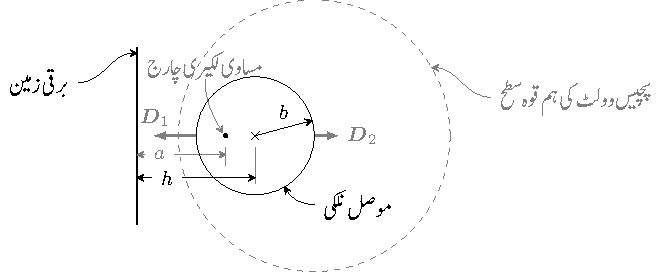
\includegraphics{figCapacitorPlainAndCylinder}
\caption{زمین کے قریب موٹی تار کا کپیسٹنس۔}
\label{شکل_کپیسٹر_زمین_کے_قریب_موٹی_تار}
\end{figure}

آئیں ان معلومات کو استعمال کرتے ہوئے لامحدود سیدھی موصل سطح  سے \عددیء{h} فاصلے پر \عددیء{b} رداس کے موصل نلکی کی کپیسٹنس حاصل کریں۔یہ صورت حال شکل \حوالہ{شکل_کپیسٹر_زمین_کے_قریب_موٹی_تار} میں دکھائی گئی ہے۔یہاں \عددیء{h} اور \عددیء{b} دئے گئے ہیں جن سے مساوات \حوالہ{مساوات_کپیسٹر_رداس_زمین_سے_فاصلہ} کی مدد سے \عددیء{a}، \عددیء{K_1} اور یوں \عددیء{V_1} معلوم کیا جا سکتا ہے۔ مساوات \حوالہ{مساوات_کپیسٹر_رداس_زمین_سے_فاصلہ} کو حل کرتے ہوئے
\begin{gather}
\begin{aligned}\label{مساوات_کپیسٹر_موصل_نلکی_زمین_متغیرات}
a&=\sqrt{h^2-b^2}\\
K_1&=\left(\frac{h+\sqrt{h^2-b^2}}{b}\right)^2
\end{aligned}
\end{gather} 
لکھا جا سکتا ہے۔اس سے
\begin{align*}
V_1=\frac{\rho_L}{2\pi\epsilon_0} \ln \frac{h+\sqrt{h^2-b^2}}{b}
\end{align*}
حاصل ہوتا ہے۔چونکہ زمین صفر وولٹ اور موصل نلکی \عددیء{V_1} وولٹ پر ہے لہٰذا ان کے درمیان \عددیء{V_1} برقی دباو ہو گا۔

شکل \حوالہ{شکل_کپیسٹر_متوازی_تار} میں مثبت تار کے \عددیء{L} لمبائی پر کل چارج \عددیء{Q=\rho_L L} پایا جاتا ہے۔ شکل \حوالہ{شکل_کپیسٹر_زمین_کے_قریب_موٹی_تار}  میں بھی برقی زمین کے اتنے ہی لمبائی پر اتنے ہی مقدار مگر منفی چارج ہو گا جبکہ \عددیء{b} رداس کے موصل نلکی پر یہی \عددیء{Q=\rho_L L} چارج ہو گا۔یوں \عددیء{L} لمبائی کے موصل نلکی اور زمین کے درمیان
\begin{align}\label{مساوات_کپیسٹر_نلکی_زمین_کپیسٹنس}
C=\frac{Q}{V_1}=\frac{2\pi\epsilon_0 L}{ \ln \frac{h+\sqrt{h^2-b^2}}{b}}=\frac{2\pi\epsilon_0 L}{\cosh^{-1} \frac{h}{b}}
\end{align}
کپیسٹنس پایا جائے گا۔

زمین سے دور کم موٹائی کے تار کی صورت میں \عددیء{h \gg b} ہو گا لہٰذا مساوات \حوالہ{مساوات_کپیسٹر_نلکی_زمین_کپیسٹنس}
\begin{align}\label{مساوات_کپیسٹر_نلکی_زمین_کپیسٹنس_ب}
C=\frac{2\pi\epsilon_0 L}{ \ln \frac{2h}{b}} \quad{h \gg b}
\end{align}
صورت اختیار کر لے گا جو نسبتاً آسان مساوات ہے۔شکل \حوالہ{شکل_کپیسٹر_متوازی_تار} میں دو تاروں کے درمیان کپیسٹنس مساوات \حوالہ{مساوات_کپیسٹر_نلکی_زمین_کپیسٹنس} کے جواب کا نصف ہو گا چونکہ مثبت تار اور زمین کے مابین کپیسٹر اور منفی تار اور زمین کے مابین کپیسٹر کو سلسلہ وار جڑا تصور کیا جا سکتا ہے۔   

کچھ حقائق مثال کی مدد سے بہتر سمجھ آتے ہیں۔آئیں مثال \حوالہ{مثال_کپیسٹر_نلکی_زمین_کپیسٹنس} کی مدد سے ایسی چند باتیں سیکھیں۔

%==================
\ابتدا{مثال}\شناخت{مثال_کپیسٹر_نلکی_زمین_کپیسٹنس}
برقی زمین کے متوازی خالی خلاء میں دس میٹر کے فاصلے پر پانچ میٹر رداس کی موصل نلکی پائی جاتی ہے جس پر پچاس وولٹ کا برقی دباو ہے۔
\begin{itemize}
\item
نلکی پر لکیری چارج کثافت حاصل کریں۔
\item
ایک میٹر لمبائی کے لئے نلکی اور زمین کے مابین کپیسٹنس حاصل کریں۔
\item
پچیس وولٹ ہم قوہ سطح کا رداس اور زمین سے اس کے مرکز کا فاصلہ حاصل کریں۔ 
\item
زمین سے ایسی لکیری چارج کثافت کا فاصلہ دریافت کریں جو ہوبہو ایسی ہی ہم قوہ سطحیں پیدا کرے گا۔
\item
نلکی پر زیادہ سے زیادہ  اور کم سے کم سطحی چارج کثافت حاصل کریں۔

\end{itemize}

حل: صورت حال شکل \حوالہ{شکل_کپیسٹر_زمین_کے_قریب_موٹی_تار} میں دکھائی گئی ہے۔
\begin{itemize}
\item
یہاں \عددیء{h=10} جبکہ \عددیء{b=5} ہیں لہٰذا مساوات \حوالہ{مساوات_کپیسٹر_موصل_نلکی_زمین_متغیرات} کی مدد سے
\begin{align*}
a&=\sqrt{10^2-5^2}=\SI{8.66}{\meter}\\
K_1&=\left(\frac{10+\sqrt{10^2-5^2}}{5}\right)^2=13.92\\
\end{align*}
حاصل ہوتے ہیں۔مساوات \حوالہ{مساوات_کپیسٹر_زمین_موٹی_تار_جزوی_مستقل} کے استعمال سے یوں
\begin{align*}
\rho_L=\frac{4\pi\epsilon_0 V_1}{\ln K_1}=\frac{50}{9 \times 10^9 \times \ln 13.92}=\SI{2.11}{\nano \coulomb \per \meter}
\end{align*}
حاصل ہوتا ہے۔
\item
مساوات \حوالہ{مساوات_کپیسٹر_نلکی_زمین_کپیسٹنس} یا کپیسٹنس کی تعریف سے فی میٹر کپیسٹنس حاصل کرتے ہیں۔
\begin{align*}
C=\frac{\rho_L L}{V_1} =\frac{2.11 \times 10^{-9} \times 1}{50}=\SI{4.22}{\nano \farad }
\end{align*}
\item
پچیس وولٹ ہم قوہ سطح کے لئے مساوات \حوالہ{مساوات_کپیسٹر_زمین_موٹی_تار_جزوی_مستقل} سے 
\begin{align*}
K_2=e^{\frac{4\pi\epsilon_0 V_2}{\rho_L}}=e^{\frac{25}{9\times 10^9 \times 2.11 \times 10^{-9}}}=3.73
\end{align*}
حاصل ہوتا ہے۔یوں مساوات \حوالہ{مساوات_کپیسٹر_رداس_زمین_سے_فاصلہ} سے پچیس وولٹ کے ہم قوہ سطح کے لئے
\begin{align*}
b&=\frac{2\times 8.66 \times \sqrt{3.73}}{3.73-1}=\SI{12.25}{\meter}\\
h&=8.66 \times \left(\frac{3.73+1}{3.73-1} \right)=\SI{15}{\meter}
\end{align*}
حاصل ہوتے ہیں۔پچیس وولٹ کے ہم قوہ سطح جس کا رداس سوا بارہ میٹر اور جو زمین سے پندرہ میٹر کے فاصلے پر ہے  کو شکل میں ہلکی سیاہی سے نقطہ دار گول دائرے سے دکھایا گیا ہے۔
\item
برقی زمین سے  \عددیء{\SI{8.66}{\meter}} فاصلے پر \عددیء{\SI{2.11}{\nano \coulomb \per \meter}} لکیری چارج کثافت کی باریک تار بالکل اسی طرز کے ہم قوہ سطحیں پیدا کرے گا۔ 
\item
کسی بھی جگہ \عددیء{\kvec{E}} کو مساوات \حوالہ{مساوات_کپیسٹر_ہم_قوہ_سطح_کارتیسی_مساوات}

\begin{align*}
V=\frac{\rho_L}{4\pi\epsilon_0} \left[\ln(x^2+(y+a)^2)-\ln(x^2+(y-a)^2)  \right]
\end{align*}
 کے ڈھلوان \عددیء{\kvec{E}=-\nabla V} سے حاصل کیا جا سکتا ہے جس سے  
\begin{align*}
\kvec{D}=\epsilon_0 \kvec{E}=-\epsilon_0\nabla V=-\epsilon_0 \left(\frac{\partial V}{\partial x}\ax+\frac{\partial V}{\partial y}\ay \right)
\end{align*}
بھی حاصل ہوتا ہے جہاں 
\begin{align*}
\frac{\partial V}{\partial x}&=\frac{\rho_L}{4\pi\epsilon_0}\left[\frac{2x}{x^2+(y+a)^2}-\frac{2x}{x^2+(y-a)^2} \right]\\
\frac{\partial V}{\partial y}&=\frac{\rho_L}{4\pi\epsilon_0}\left[\frac{2(y+a)}{x^2+(y+a)^2}-\frac{2(y-a)}{x^2+(y-a)^2} \right]
\end{align*}
کے برابر ہیں۔

چونکہ موصل کے سطح پر \عددیء{\kvec{D}} عمودی ہوتا ہے اور اس کی قیمت سطحی چارج کثافت کے برابر ہوتی ہے لہٰذا ہم موصل نلکی پر برقی زمین کے قریبی
 جانب \عددیء{\kvec{D}_1} اور اس سے دور جانب \عددیء{\kvec{D}_2} کی قیمت حاصل کرتے ہیں۔انہیں شکل \حوالہ{شکل_کپیسٹر_زمین_کے_قریب_موٹی_تار} میں دکھایا گیا ہے۔زمین سے نلکی کا قریبی فاصلہ \عددیء{h-b=\SI{5}{\meter}} ہے۔یوں  \عددیء{x=0} اور \عددیء{y=5} ہو گا جس سے
\begin{align*}
\frac{\partial V}{\partial x}&=\frac{\rho_L}{4\pi\epsilon_0}\left[\frac{2 \times 0}{0^2+(5+8.66)^2}-\frac{2 \times 0}{0^2+(5-8.66)^2} \right]=0\\
\frac{\partial V}{\partial y}&=\frac{\rho_L}{4\pi\epsilon_0}\left[\frac{2(5+8.66)}{0^2+(5+8.66)^2}-\frac{2(5-8.66)}{0^2+(5-8.66)^2} \right]=\frac{0.693 \rho_L}{4\pi\epsilon_0}
\end{align*}
حاصل ہوتے ہیں۔یوں
\begin{align*}
\kvec{D}_{1}=-\frac{0.693 \rho_L}{4\pi} \ay
\end{align*}
ہو گا۔زمین سے دور نلکی پر \عددیء{x=0} اور \عددیء{y=h+b=10+5=\SI{15}{\meter}} ہیں جس سے
\begin{align*}
\frac{\partial V}{\partial x}&=\frac{\rho_L}{4\pi\epsilon_0}\left[\frac{2 \times 0}{0^2+(15+8.66)^2}-\frac{2\times 0}{0^2+(15-8.66)^2} \right]=0\\
\frac{\partial V}{\partial y}&=\frac{\rho_L}{4\pi\epsilon_0}\left[\frac{2(15+8.66)}{0^2+(15+8.66)^2}-\frac{2(15-8.66)}{0^2+(15-8.66)^2} \right]=-\frac{0.231\rho_L}{4\pi\epsilon_0}
\end{align*}
یا
\begin{align*}
\kvec{D}_{2}=\frac{0.231\rho_L}{4\pi} \ay
\end{align*}
حاصل ہوتا ہے۔دونوں جوابات سے ظاہر ہے کہ بہاو کا اخراج سطح کے عمودی ہے۔یوں موصل نلکی پر
\begin{align*}
\rho_{S\textup{قریبی}}&=\frac{0.693 \rho_L}{4\pi}\\
\rho_{S\textup{دور}}&=\frac{0.231 \rho_L}{4\pi}
\end{align*}
پایا جائے گا۔یاد رہے کہ قریبی جانب منفی جواب کا مطلب ہے کہ اخراج زمین کی جانب ہے جبکہ دور جانب مثبت جواب کا مطلب ہے کہ اخراج \عددیء{\ay} جانب ہے۔دونوں جانب اخراج ہی ہے لہٰذا سطحی چارج کثافت دونوں جگہوں پر مثبت ہی ہے۔  

\end{itemize}
\انتہا{مثال}
%================

اس مثال سے صاف ظاہر ہے کہ نلکی کا چارج بالکل اس طرح عمل کرتا ہے جیسے برقی زمین سے  \عددیء{\SI{8.66}{\meter}} فاصلے پر باریک چارج بردار تار جس پر  \عددیء{\SI{2.11}{\nano \coulomb \per \meter}} پایا جاتا ہو۔نلکی سے پیدا ہم قوہ سطحیں اسی فرضی لکیری چارج کثافت کے تار سے حاصل کی جاتی ہیں۔

%=======================
\ابتدا{مشق}
مساوات \حوالہ{مساوات_کپیسٹر_موصل_نلکی_زمین_متغیرات} کو ثابت کریں۔
\انتہا{مشق}
%=======================

%==============================
\section*{سوالات}

\ابتدا{سوال}
\عددیء{N(0,0,2)} سے گزرتی \عددیء{y} محدد کے متوازی لکیری چارج کثافت
\begin{align*}
\rho_L=\SI{5}{\nano \coulomb \per \meter}  \quad \quad (-\infty < y < \infty, x=0,z=2)
\end{align*} 
سے \عددیء{M(5,3,1)} پر \عددیء{\kvec{D}} حاصل کریں۔

جواب:\عددیء{\kvec{D}=\tfrac{5\times 10^{-9}(5\ax-1\az)}{2 \pi \times 26}}
\انتہا{سوال}
%==========
\ابتدا{سوال}
لامحدود موصل زمینی سطح \عددیء{z=0}  رکھتے ہوئے  مندرجہ بالا سوال کو دوبارہ حل کریں۔

جواب:\عددیء{\kvec{D}=\tfrac{5\times 10^{-9}(40\ax-112\az)}{2 \pi \times 884}}
\انتہا{سوال}
%====
\ابتدا{سوال}
\عددیء{N(0,0,2)} سے گزرتی \عددیء{y} محدد کے متوازی لکیری چارج کثافت
\begin{align*}
\rho_L=\SI{5}{\nano \coulomb \per \meter}  \quad \quad (-\infty < y < \infty, x=0,z=2)
\end{align*} 
پایا جاتا ہے جبکہ \عددیء{z=0} پر لامحدود موصل زمینی سطح موجود ہے۔سطح کے \عددیء{M(5,3,0)} مقام پر سطحی چارج کثافت حاصل کریں۔

جواب: \عددیء{\SI{-0.1097}{\nano \coulomb \per \meter \squared}}
\انتہا{سوال}
%=======
\ابتدا{سوال}
مشق \حوالہ{مشق_کپیسٹر_نیم_موصل_موصلیت} میں \عددیء{\SI{300}{\kelvin}} درجہ حرارت پر  سلیکان اور جرمینیم کے مستقل دئے گئے ہیں۔اگر سلیکان میں المونیم کا ایک ایٹم فی  \عددیء{\num{1e7}} سلیکان ایٹم  ملاوٹ شامل کی جائے تو سیلکان کی موصلیت کیا ہو گی۔سلیکان کی تعدادی کثافت \عددیء{\num{5e28}} ایٹم فی مربع میٹر ہے۔(ہر ملاوٹی المونیم کا  ایٹم ایک عدد آزاد خول پیدا کرتا ہے جن  کی تعداد مشق میں دئے خالص سلیکان میں آزاد خول کی تعداد سے بہت زیادہ ہوتی ہے لہٰذا ایسی صورت میں موصلیت صرف ملاوٹی ایٹموں کے پیدا کردہ آزاد خول ہی تعین کرتے ہیں۔) 

جواب: \عددیء{\SI{800}{\siemens \per \meter}}
\انتہا{سوال}
%======
\ابتدا{سوال}
صفحہ \حوالہصفحہ{مثال_کپیسٹر_نقطہ_چارج_سے_لامحدود_سطح_میں_پیدا_کثافت} پر مثال \حوالہ{مثال_کپیسٹر_نقطہ_چارج_سے_لامحدود_سطح_میں_پیدا_کثافت} میں لامحدود موصل سطح \عددیء{z=0} میں \عددیء{(0,0,z)} پر پائے جانے والے نقطہ چارج \عددیء{Q} سے پیدا سطحی چارج کثافت \عددیء{\rho_S} حاصل کیا گیا۔موصل سطح میں پائے جانے والا کل چارج سطحی تکمل سے حاصل کریں۔

جواب: \عددیء{-Q} 
\انتہا{سوال}
%========================
\ابتدا{سوال}
صفحہ \حوالہصفحہ{مساوات_کپیسٹر_موصل_آزاد_چارج_کثافت} پر تانبے کے ایک مربع میٹر میں کل آزاد چارج مساوات \حوالہ{مساوات_کپیسٹر_موصل_آزاد_چارج_کثافت} میں حاصل کیا گیا۔ایک ایمپئیر کی برقی رو کتنے وقت میں اتنے چارج کا اخراج کرے گا۔

جواب: چار سو اکتیس \عددیء{(431)} سال۔ 
\انتہا{سوال}
%=========================

\ابتدا{سوال}
مساوات \حوالہ{مساوات_کپیسٹر_نلکی_زمین_کپیسٹنس} میں  \عددیء{\ln \frac{h+\sqrt{h^2-b^2}}{b}=\cosh^{-1} \frac{h}{b}} لکھا گیا ہے۔اسے ثابت کریں۔
\انتہا{سوال}
%===========

\ابتدا{سوال}
پانچ میٹر رداس کی موصل نلکی کا محور برقی زمین سے تیرہ میٹر پر ہے۔نلکی پر ایک سو وولٹ کا برقی دباو ہے۔
\begin{itemize}
\item
ایسی لکیری چارج کثافت کا زمین سے فاصلہ اور اس کا \عددیء{\rho_L} حاصل کریں جو ایسی ہم قوہ سطح  پیدا کرے۔
\item
موصل نلکی سے پیدا پچاس وولٹ کے ہم قوہ سطح کا رداس اور اس کے محور کا زمین سے فاصلہ دریافت کریں۔
\item
نلکی پر زمین کے قریب اور اس سے دور سطحی چارج کثافت حاصل کریں۔
\end{itemize} 

جوابات:\عددیء{\SI{12}{\meter}}، \عددیء{\SI{3.46}{\nano \coulomb \per \meter}}، \عددیء{\SI{13.4}{\meter}}، \عددیء{\SI{18}{\meter}}، \عددیء{\SI{1.65}{\pico \farad \per \meter \squared}} اور \عددیء{\SI{0.73}{\pico \farad \per \meter \squared}}

\انتہا{سوال}
%=============

